\documentclass[a4paper,12pt, oneside]{book}
\usepackage{bm}
\usepackage{siunitx}
\usepackage{cases}
\usepackage[english]{babel}
\usepackage[dvipdfmx]{graphicx}
\usepackage{subfig} 
\columnsep 3zw
\renewcommand\baselinestretch{0.8} 
\topmargin -1.5cm        % read Lamport p.163
\oddsidemargin -0.04cm  % read Lamport p.163
\evensidemargin -0.04cm  % same as oddsidemargin but for left-hand pages
\textwidth 16.59cm
\textheight 23.50cm 
% \pagestyle{empty}       % Uncomment if don't want page numbers
\parskip 7.2pt           % sets spacing between paragraphs
% \renewcommand{\baselinestretch}{1.5} 	% Uncomment for 1.5 spacing between lines
\hyphenpenalty=2000\relax
\exhyphenpenalty=2000\relax
\sloppy
\title{\Large Graduate School of Sciences and Technology for Innovation, Yamaguchi University\\[1cm]
Division of Fundamental Sciences\\[3cm]
\huge A Computational Model of Cell Migration of Fish Keratocytes\\[5cm]
}
\author{Yu Tokunaga}
\date{\Large \today}
\begin{document}
\pagenumbering{roman}
\maketitle
\setcounter{page}{1}
\tableofcontents
\chapter{Introduction}
\pagenumbering{arabic}
\setcounter{page}{1}
%問題提起
{\it Amoeba proteus},  a common ameba cell, migrates by stretching pseudopodia with changing  its cell shape continuously.
In contrast, fish keratocytes usually show a circular shape; however, they change their shape to a half-moon shape when they begin migration. This phenomenon suggests that the deformation of the cell shape is a key feature to realize cell migration of keratocytes.

%いかに不思議か(問題点を具体化)
As evidence that AP is important for cell deformation, it has been reported that a dense network of actin molecules regulates cell deformation\cite{svitkina1997analysis}.
Previous studies have reported that during cell migration actin molecules extend their head toward the cell membrane by actin polymerization (AP), which has been suggested as a source of the deformation of the cell membrane and the propulsive force of the cell.
As evidence that AP is important for cell deformation, it has been reported that a dense network of actin molecules regulates cell deformation.
The actin retrograde flow (ARF) that pulls the actin molecules back toward the stress fiber (SF), a bundle of actin fibers spreading from side to side of the rear part of the cell, has also been reported\cite{swaminathan2017actin}.

%目的
The purpose of this research is to clarify the mechanism that forms a half-moon shape by physical simulation experiments considering intracellular mechanism.

%本稿の構成                    
The structure of this paper is as follows. In Chapter 2, we introduce previous work on the molecular mechanism of cell migration of keratinocytes. In chapter 3 we will explain our method of simulation experiments. Section 4 shows the results of simulation experiments. In the last chapter, we will discuss conclusions and future prospects for the purpose.


%第2章
\chapter{Keratocytes}
\section{Characteristics of Cell Migration of Keratocytes}
\begin{figure}[tbp]
\centering
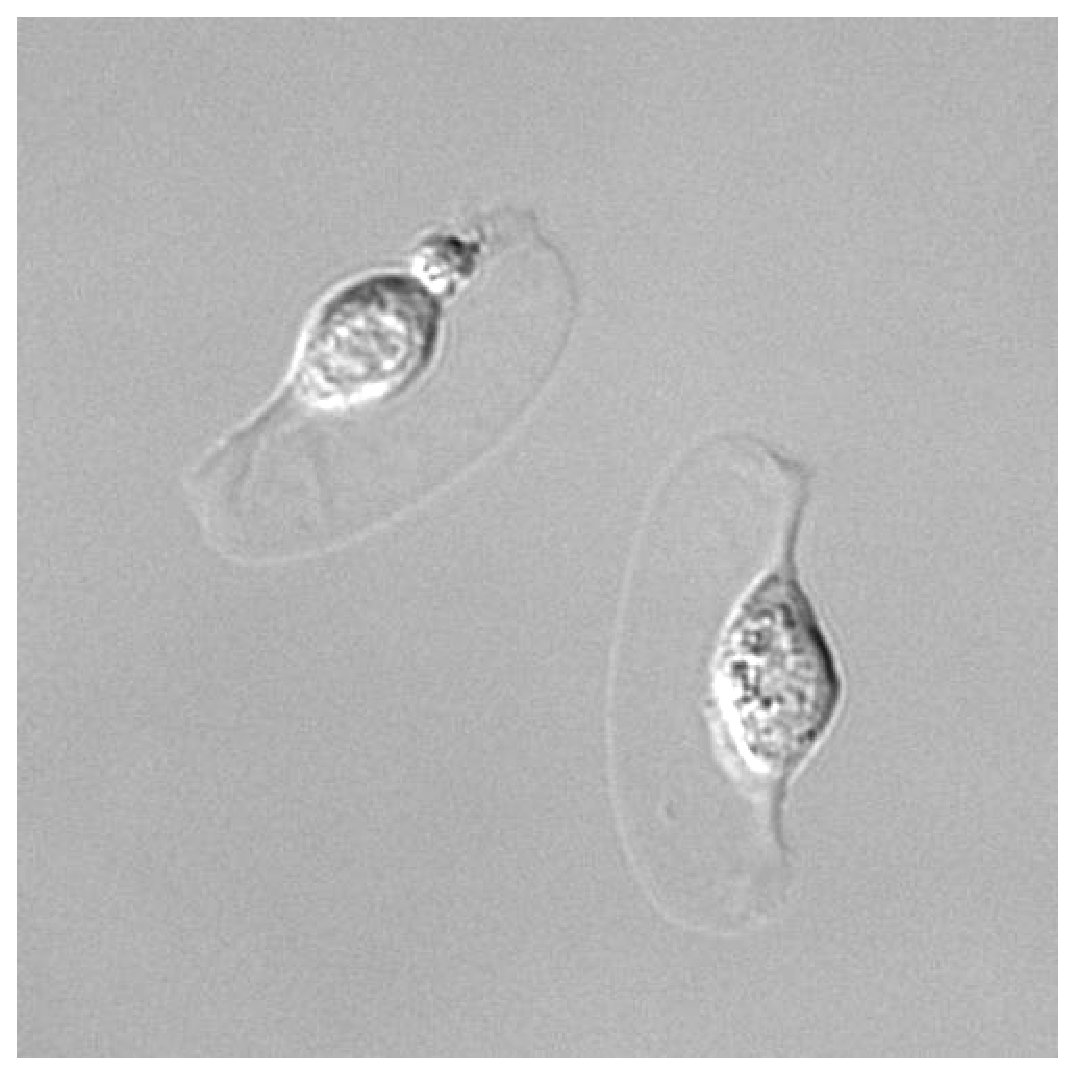
\includegraphics[scale=0.4]{kera.eps}
\caption{Keratocytes during cell migration.(Source: Takako Tanaka, Iwadate Lab).}
\label{fig:kera}
\end{figure}

%ケラトサイトの自己紹介
A keratocytes, a migratory fish epidermal cell, is a wound healing cell about \SI{70}{\mu m}  in size.
When a fish injures, keratocytes begin migration toward the injured position toward  the wound by the speed of about one body length in one minute.
The locomotion of keratocytes is a kind of amoeboid movements;
however, it is different from typical amoeba movement at the point that they moves  with keeping a half-moon shape. 

%参考文献
%アクチン分子
The protruding events of cell migration are thought to be caused by actin polymerization (AP)\cite{svitkina1997analysis}.
AP is that actin molecules which are cytoskeletons overlap to form fibrous actin (F-actin).
%cell migration と actinの重合と脱重合の関連
There is depolymerization in the opposite phenomenon of AP.
The opposite of AP, the phenomenon that actin molecule separates from F-actin is called depolymerization.
The actin molecule depolymerizes with AP and forms a dense network and pushes the cell membrane from the inside.
%ARFとSFの紹介
There are not only actin molecules but also myosin molecules in the cell membrane.
When actin molecule and myosin molecule are bound, it becomes actomyosin, and a bundle of actomyosin is called a stress fiber (SF).
The actin retrograde flow (ARF) that pulls the actin molecules back toward the SF has also been reported \cite{swaminathan2017actin}.
%cell migrationとARFとSFの関連
Although details on ARF are not clarified, it is thought that SF attracts forward actin molecule towards SF \cite{nakata2016role}.
The network of actin molecules moves by AP and ARF to promote cell membrane deformation.
In addition, Okimura et.al reported that SF plays a role of wheels in cell migration \cite{okimura2018rotation}.
In the cell migration when SF was removed, the migration speed decreased and the left and right balance disintegrated.
This also indicates that SF is important for cell migration.

It has been reported that morphogenesis of morphology was observed even after removing the nucleus \cite{asano2004keratocyte}.
Hence, it was suggested that the cell migration of the keratocyte is due to a physical factor, not genetic information.


\section{Molecular Mechanism of Cell Migration}
A cell has a structure called a cytoskeleton. The cytoskeleton is like bones for humans, but in contrast to static human bones, the cytoskeleton is dynamic and is an important organelle that maintains the shape of the cell. The main component of the cytoskeleton is the actin molecule. As the actin molecule polymerizes and depolymerizes, the shape of the cell membrane changes. The actin molecule is elongated by polymerization in the cell membrane but retreats in the direction opposite to the elongation direction by the bundle of actomyosin called stress fiber. This phenomenon is called actin retrograde flow, and it is not clear what kind of role it plays in cell migration. The cell membrane extruded by polymerization of the actin molecule becomes the pseudopodia and adheres to the substrate at the advancing position. Thereafter, the adhesion between the substrates of the rear cell membrane is released and dragged forward. By repeating this cycle, cell migration mechanism is formed.

It is a common fact even in keratocytes that the cell membrane is deformed by actin molecule polymerization. In the simulation experiment described in the next chapter, we investigate how the cell membrane forms a half moon shape when actin molecule polymerization acts on the cell membrane.


\chapter{Simulation Methods}
\section{Simulation Methods of Cell Membrane}
%初期配置の話
In the computer simulation of this study, the cell membrane was modeled by a network of simple particles interacting with each other and placed on a cylindrical surface as an initial condition.
Each particle of the membrane was assumed to receive elastic force from neighboring particles and repulsive force from actin molecules.
The equation of motion of the cell membrane molecule is assumed as follows.

\begin{equation}
m\frac{d^2\bm{x}_i}{dt^2} = \bm{F}^m_i +  \bm{F}^a_i - \eta \frac{d\bm{x}_i}{dt}
\end{equation}

where  $\bm{x}_i$ is the position vector of the membrane molecule, $m$ is the mass of the particle, $\eta=8.9\times10^{-6}\si{~kg/s}$ is the viscous coefficient, $\bm{F}^m_i$ and $\bm{F}^a_i$ is the force received from the neighboring particles and  the repulsive force from actin molecules.
The force  $\bm{F}^m_i$ was assumed as an elastic force:
\begin{equation}
\bm{F}^m_i = \sum_{i \in I_j}  -k((\bm{x}_j -\bm{x}_i )-\bm{l}_{ij} )
\end{equation}
where $k$ is a spring constant, $\bm{l}_{ij}$ is the natural length between the $i$-th and $j$-th membrane particles, and $I_j$ represents the set of particles that interacts with particle $j$.
The natural length between particles were determined by the distance  at the initial state.
The force $\bm{F}^a_i$ received from an actin particle was assumed to be a  repulsive force:
\begin{equation}
\bm{F}^a_i = \sum_{\{ \forall i | \| \bm{x}_j - \bm{B}_i \|<D_2\}} \frac{s}{\|\bm{x}_j -\bm{B}_i \|} \frac{\bm{x}_j -\bm{B}_i }{\|\bm{x}_j -\bm{B}_i \|}
\end{equation}
where $s$ is a constant that determines the strength of the repulsive force, and $D_2$ is a distance range  the  force prepared to decrease the calculation amount.

\section{Simulation Methods of Actin Molecules}
\subsection{Actin Polymerization}
An actin molecule has polarity: one end which elongates by  polymerization is called barbed-end, and the other end is called pointed-end.
Since the frequency of polymerization is high in a region where actin molecules are dense \cite{svitkina1997analysis}, the polymerization rate was assumed to be  proportional to the actin concentration.
The filament formed by actin polymerization is called F-actin.
F-actin was expressed by a simple  rod in the simulation. 
As an initial condition the length of each rod was zero and he direction of the actin polymerization $\bm{L}_i$ was  randomly determined.
The elongation of the F-actin by the polymerization is modeled by
\begin{equation}
\bm{B}_i \gets \bm{P}_i + f^p(c)\bm{L}_i \cdot dt
\end{equation}
where $\bm{B}_i$ and $\bm{P}_i$ are barbed end and pointed end of the F-actin, respectively, and $f^p(c) = 5.0 \cdot \exp{\frac{c}{10.0}}$ expresses the frequency of actin polymerization as a function of actin concentration $c$.
$c$ measures for each region obtained by dividing the plane of the simulation space into a lattice shape.
The frequency of depolymerization decreases in an actin dense area and the depolymerization was expressed  as follows.
\begin{equation}
\bm{P}_i \gets \bm{P}_i + f^d(c)\bm{L}_i \cdot dt
\end{equation}
where $f^d(c) = \frac{5.0}{c}$ represents the frequency of depolymerization. 
The actin polymerization and depolymerization was simulated by a probability  \[p_i(c) = c_i = \frac{a_i}{N}\] at each step, where $p_i(c)$ is the probability that depends on the concentration $c_i$ in $i$-th region, $a_i$ is the number of actin in $i$-th region, and $N$ is the total number of actin.
In this simulation, the space where a virtual cell was simulated was divided into $3600$ regions $(i = 1,...3600$).

There is a possibility that the actin molecule protrudes from the cell membrane by polymerization in a random direction.
The actin molecule in the region of low actin molecule density disappears and regenerates near the cell membrane.
The new polymerization direction of the actin molecule is randomly determined.

\subsection{Actin Retrograde Flow}
Because the function and underlying mechanism of the ARF have not been known in detail, we simulated the ARF under some assumptions. The ARF is a movement of F-actins toward the  stress fiber which is a bundle of actin fibers aligning from side to side in the rear side of keratocytes. 

At first, we assumed the ARF as the retraction of the actin molecules toward the leftmost point of the cell, i.e., the position of the membrane particle with the smallest x coordinate, which we call the reference point. The retraction of the actin molecule by the ARF was expressed by the following equation:
\begin{numcases}
  {}
  \bm{B}_i \gets \bm{B}_i - \alpha \frac{ \bm{B}_i - \bm{E}_0}{{\| \bm{B}_i - \bm{E}_0 \|}^w} & \\
   \bm{P}_i \gets \bm{P}_i - \beta \frac{ \bm{P}_i - \bm{E}_0}{{\| \bm{P}_i - \bm{E}_0 \|}^w} &
\end{numcases}
where $\bm{E}_0$ is the reference point, and $\alpha$ and $\beta$ are constants that determines the strength of the ARF.
$w$ is a parameter indicating the effect of distance between actin molecule and cell membrane molecule on retraction strength of the ARF.
When $w=2$, the closer the intermolecular distance is, the stronger is pulled. When $w=1$, all actin molecules are equally pulled irrespective of the intermolecular distance.

Second, we assumed that another reference points $\bm{E}_1$ and $\bm{E}_2$ are proposed.
Hence, two pattern experiments are performed with one and two ARF reference points.
As shown in the figure, the reference points $\bm{E}_1$ and $\bm{E}_2$ are positioned at 1/5 of the cell membrane.
The reference points  $\bm{E}_1$ and $\bm{E}_2$ are located 1/5 rearward of the cell membrane. ARF was expressed by contraction of actin molecule to the two points.
In this case the retraction by the ARF was expressed as follows:
\begin{numcases}
  {}
  \bm{B}_i \gets \bm{B}_i - \gamma \left( \frac{ \bm{B}_i - \bm{E}_1 }{{\| \bm{B}_i - \bm{E}_1 \|}^w} + \frac{ \bm{B}_i - \bm{E}_2}{{\| \bm{B}_i - \bm{E}_2 \|}^w} \right)& \\
   \bm{P}_i \gets \bm{P}_i - \delta \left( \frac{ \bm{P}_i - \bm{E}_1 }{{\| \bm{P}_i - \bm{E}_1 \|}^w} + \frac{ \bm{P}_i - \bm{E}_2}{{\| \bm{P}_i - \bm{E}_2 \|}^w}  \right) &
   \label{eq:arf}
\end{numcases}
where $\gamma$ and $\delta$ are constants that determines the strength of the ARF.

\section{Initial Condition}
\begin{figure}[tbp]
\centering
 \subfloat[]{%
  \begin{tabular}{c}
   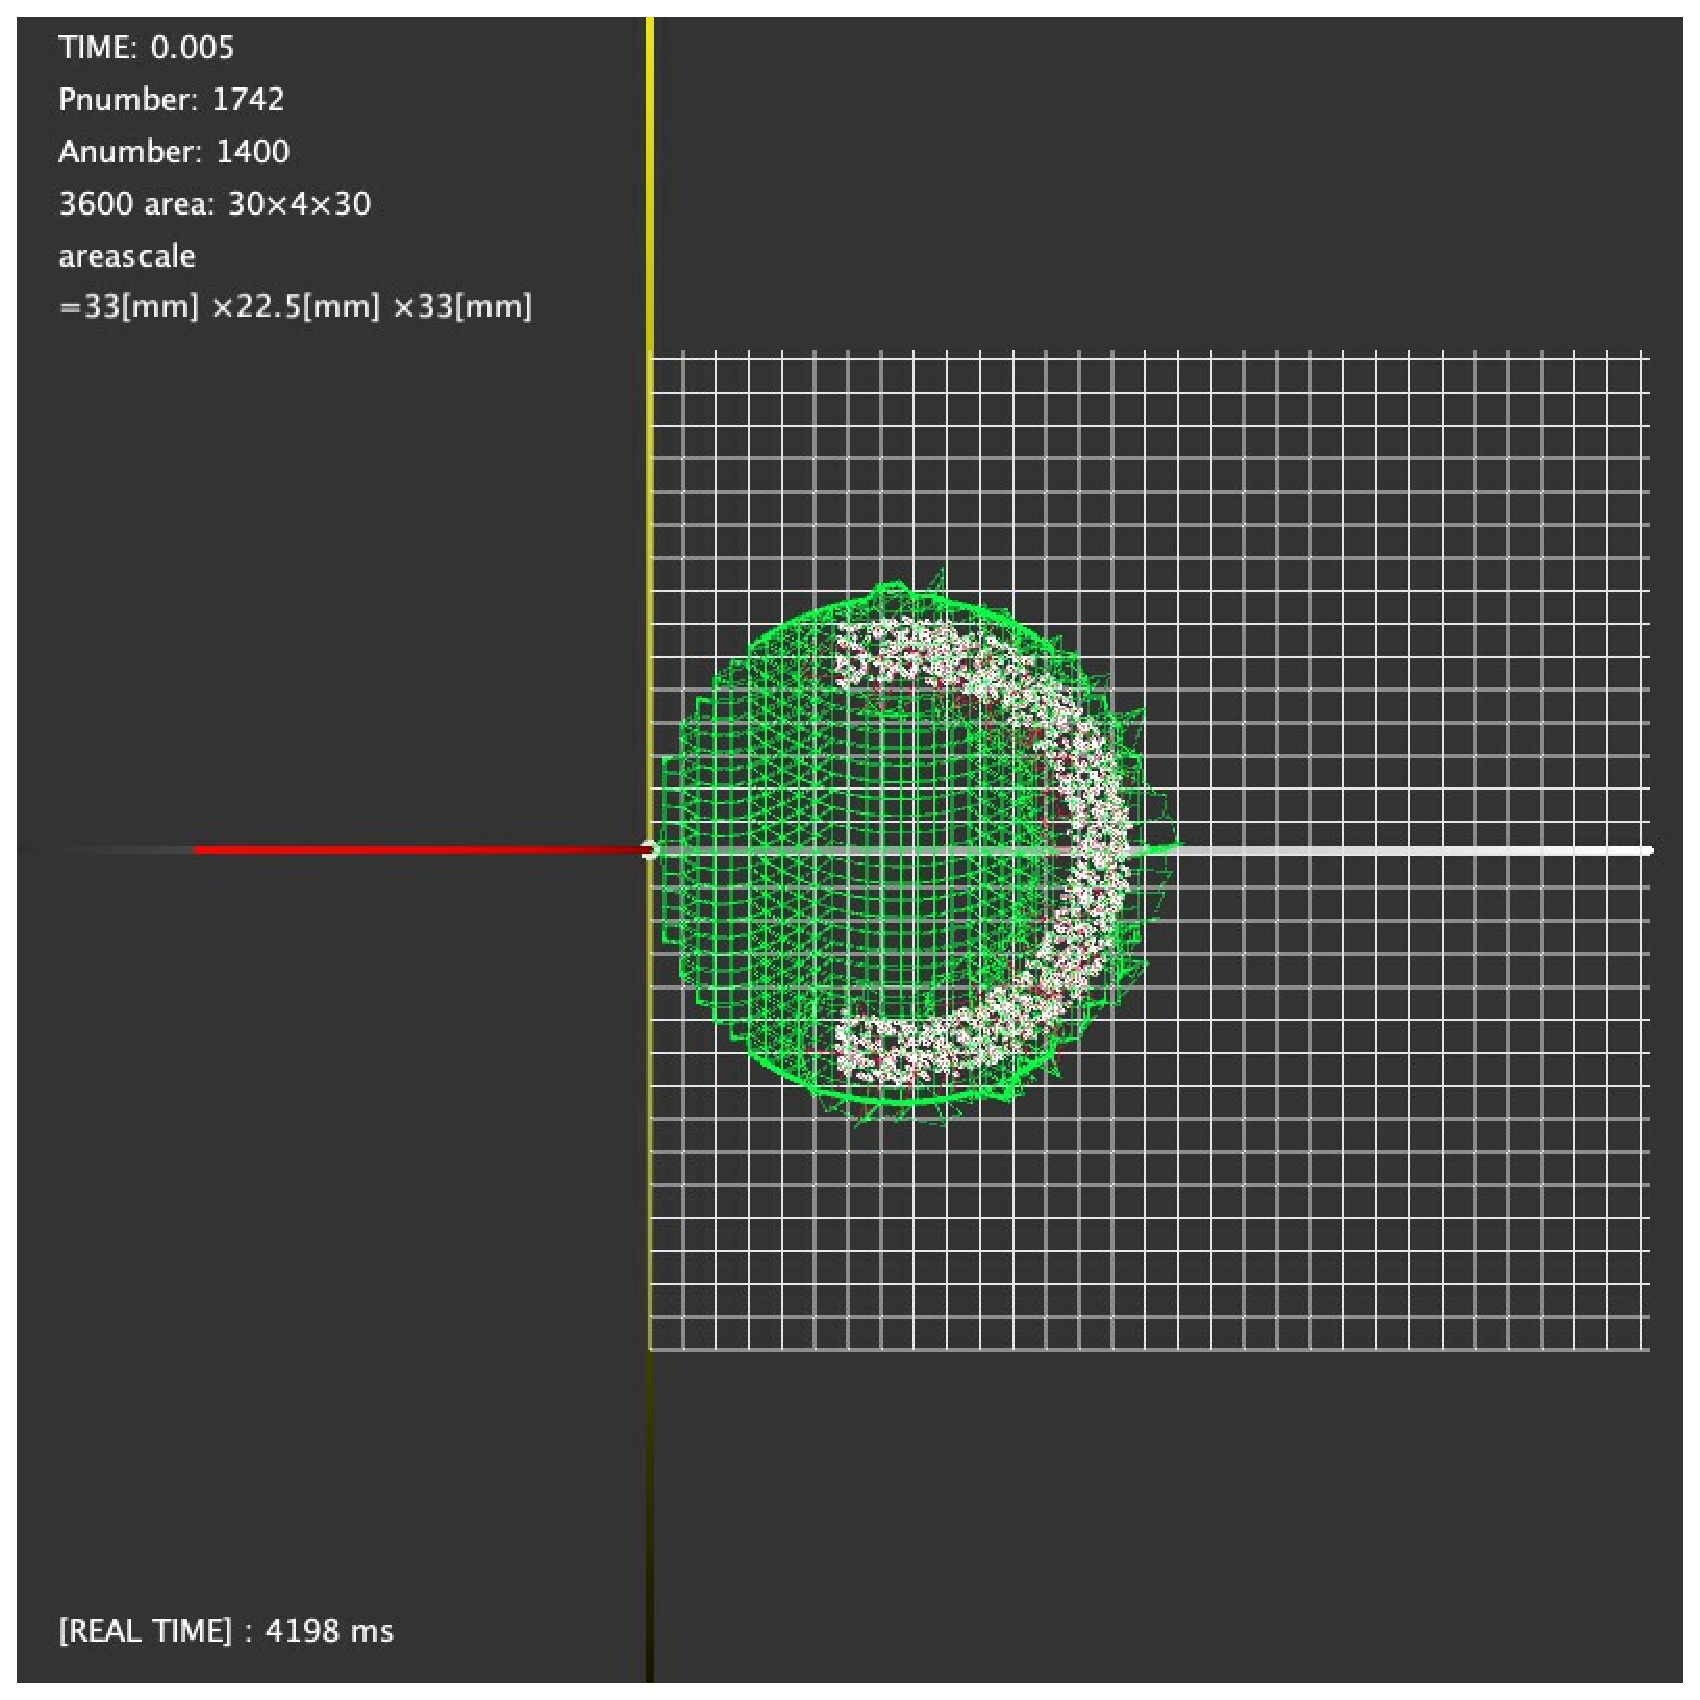
\includegraphics[width=5cm]{top.eps} 
  \end{tabular}
 }%
 \subfloat[]{%
  \begin{tabular}{c}
   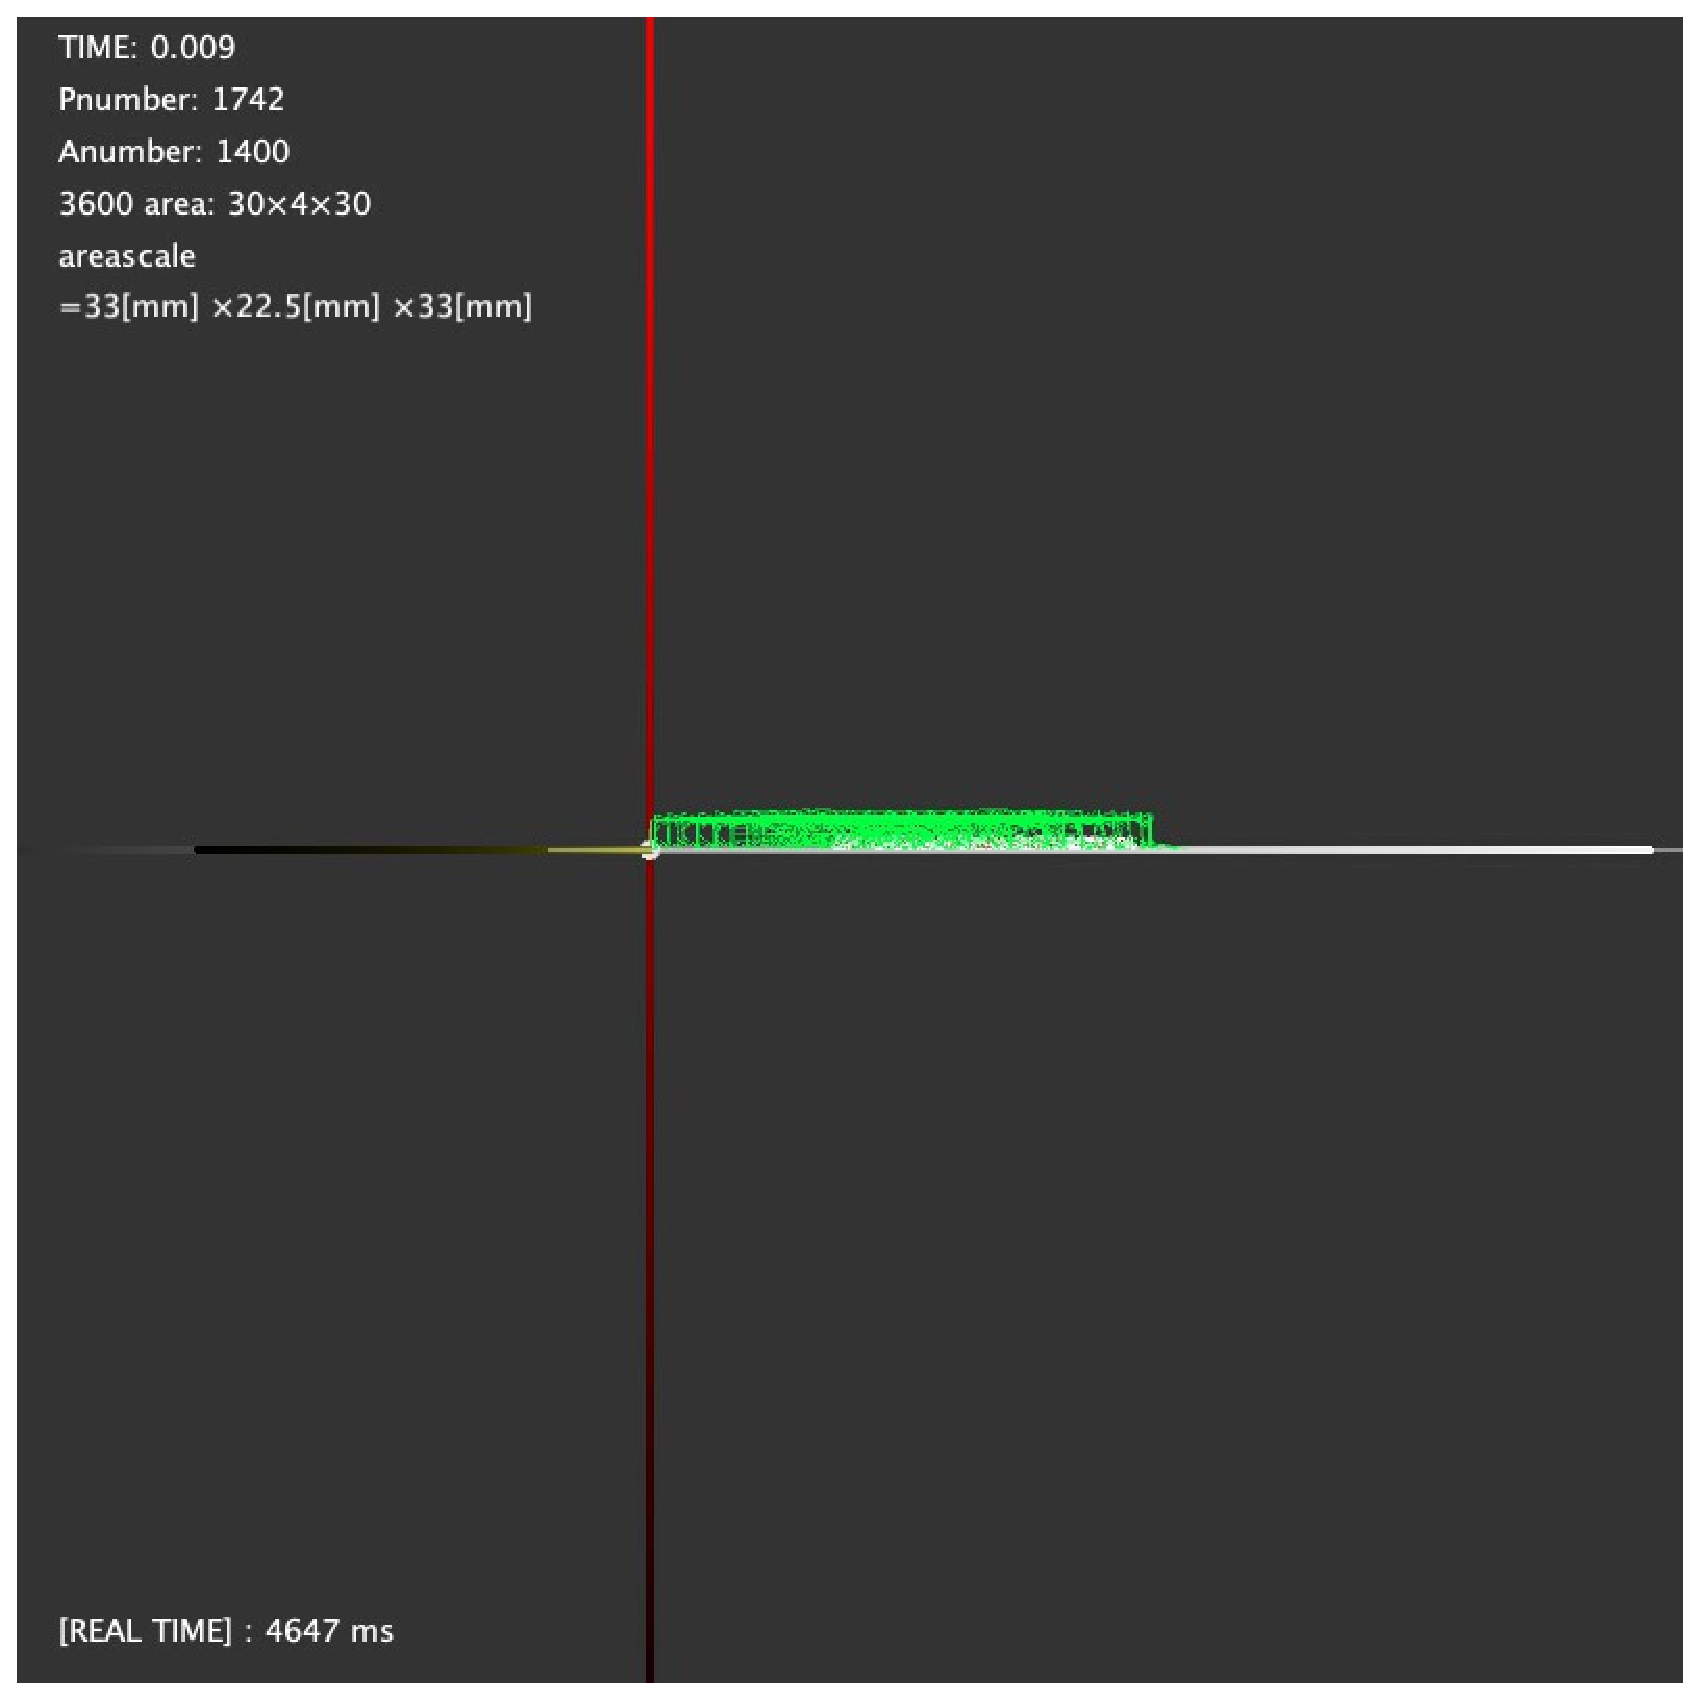
\includegraphics[width=5cm]{side.eps} 
  \end{tabular}
 }%
  \caption{Initial state. (a)~Top view. Green lines and white dots show actin molecules and membrane particles, respectively. (b)~Side view.}
 \label{fig:ini}
\end{figure}
The number of actin molecules and membrane particles were 3000 and 2000, respectively, in the computer simulation.
The positions of membrane particles were updated every step of the numerical computation and the positions of actin molecules were updated every 10 time steps.

Fig. \ref{fig:ini} shows the initial state of the virtual cell of  the computer simulation.
The initial arrangement of the actin molecule is a U-shaped area excluding the rear of the cell (Fig. \ref{fig:ini}).
The membrane molecules are placed on the surface of the cylinder and not inside.

\section{Reduction in Calculation Amount}
%細胞膜のはなし
Calculating the distance between membrane molecules in all steps increases the computational complexity.
Therefore, when calculating the cell membrane model, the distance between the cell membrane molecules stored in advance was referred to.
In the initial state, the index information of the adjacent cell membrane molecules was stored.
This method can be adopted because the position information adjacent does not change regardless of how much the interparticle distance changes.

%エリアわけ
Likewise, if the distance between the cell membrane molecule and the actin molecule is calculated in all steps, the process becomes heavy.
Unlike the case of intermolecular molecules, the index information of nearby molecules changes in the case of actin molecule and cell membrane molecules.
For this reason, the simulation space was divided into areas in mesh form, and index information of molecules in the same area was saved.


\chapter{Results and Discussion}
\section{Simulation Results}
\subsection{Role of Actin Retrograde Flow}
%SF、距離非依存
\begin{figure}[tbp]
 \subfloat[]{%
  \begin{tabular}{c}
   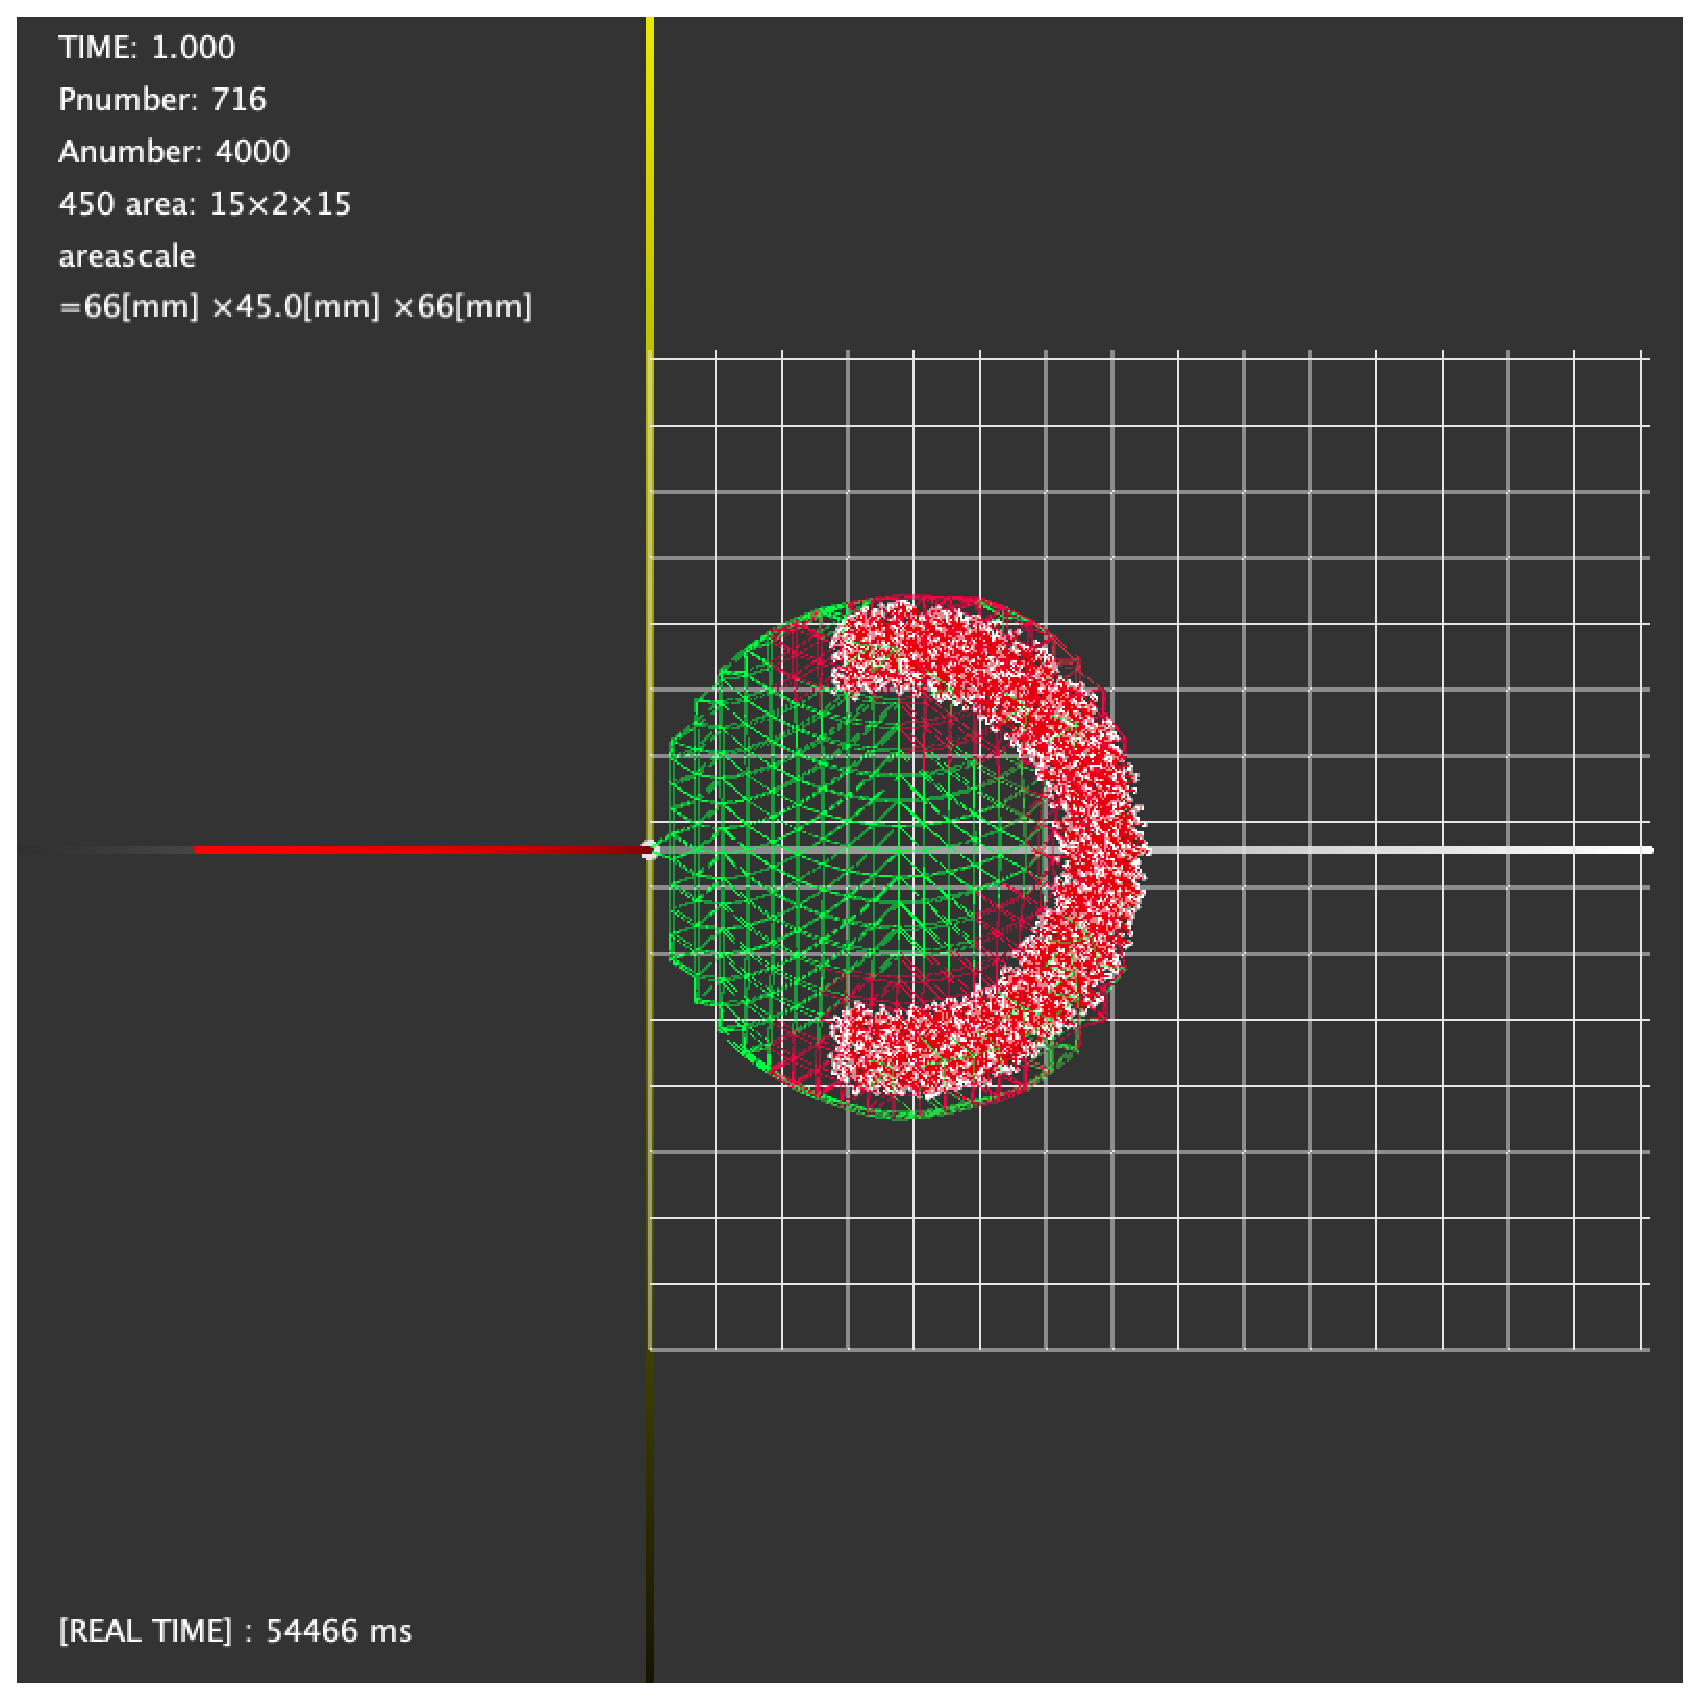
\includegraphics[width=5cm]{top10_darf.eps} 
  \end{tabular}
 }%
 \subfloat[]{%
  \begin{tabular}{c}
   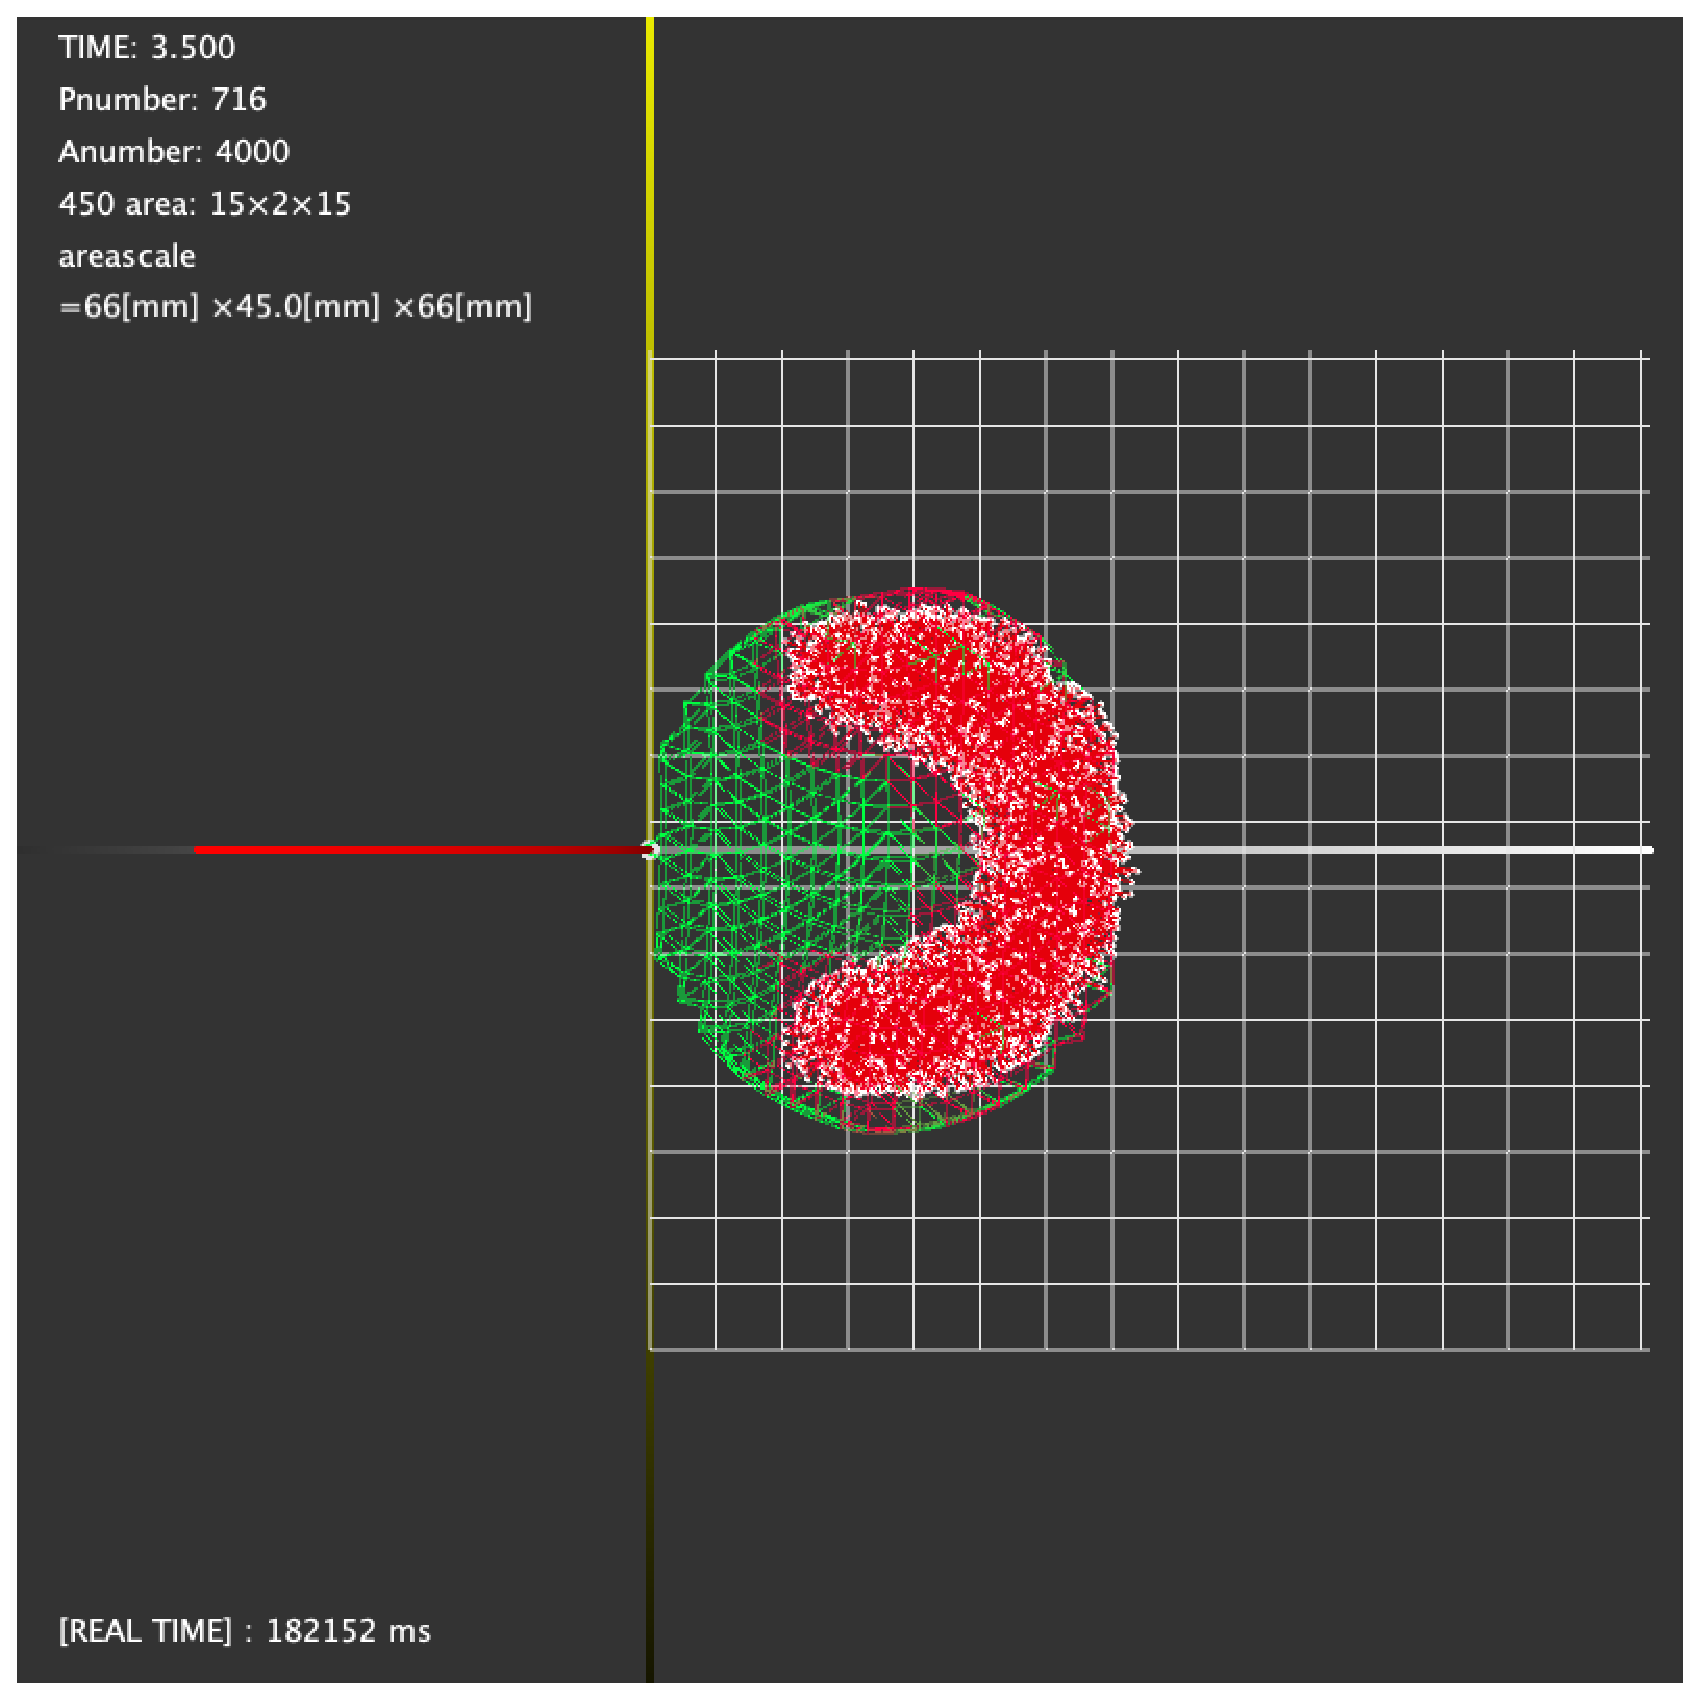
\includegraphics[width=5cm]{top35_arf.eps} 
  \end{tabular}
 }%
 \subfloat[]{%
  \begin{tabular}{c}
   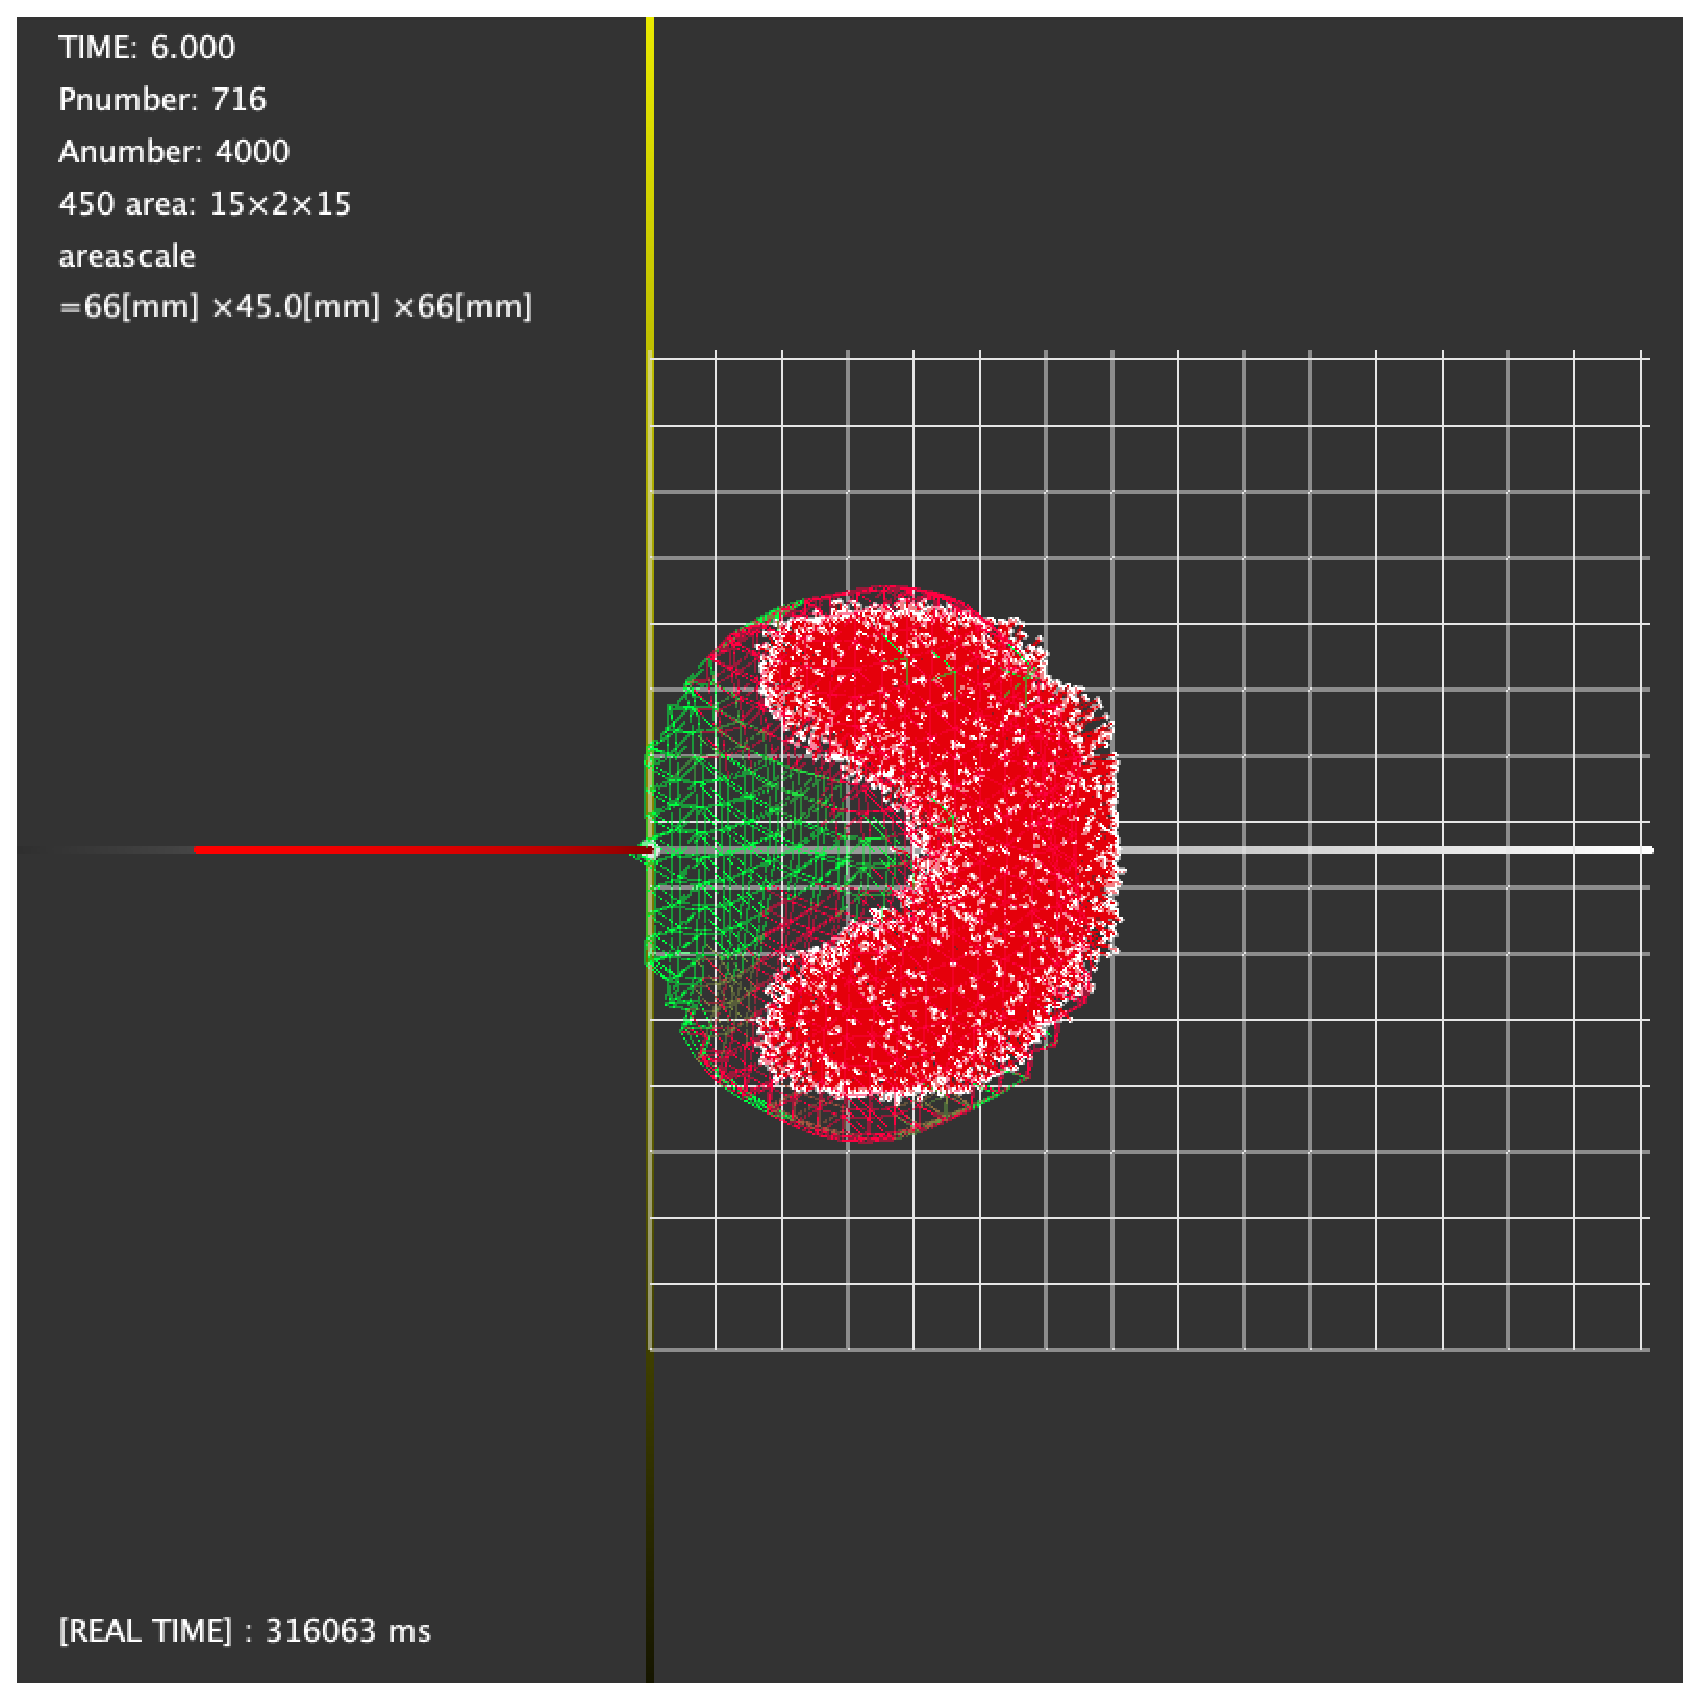
\includegraphics[width=5cm]{top60_arf.eps} 
  \end{tabular}
 }%
 \caption{Simulation results when the amplitude of the retraction by the ARF is independent of the distance. time $t = 1.0, 3.5, 6.0 [s]$. Green lines show the cell membrane, and red dots show F-actin.}
 \label{fig:res0}
\end{figure}

%SF、距離依存
\begin{figure}[tbp]
 \subfloat[]{%
  \begin{tabular}{c}
   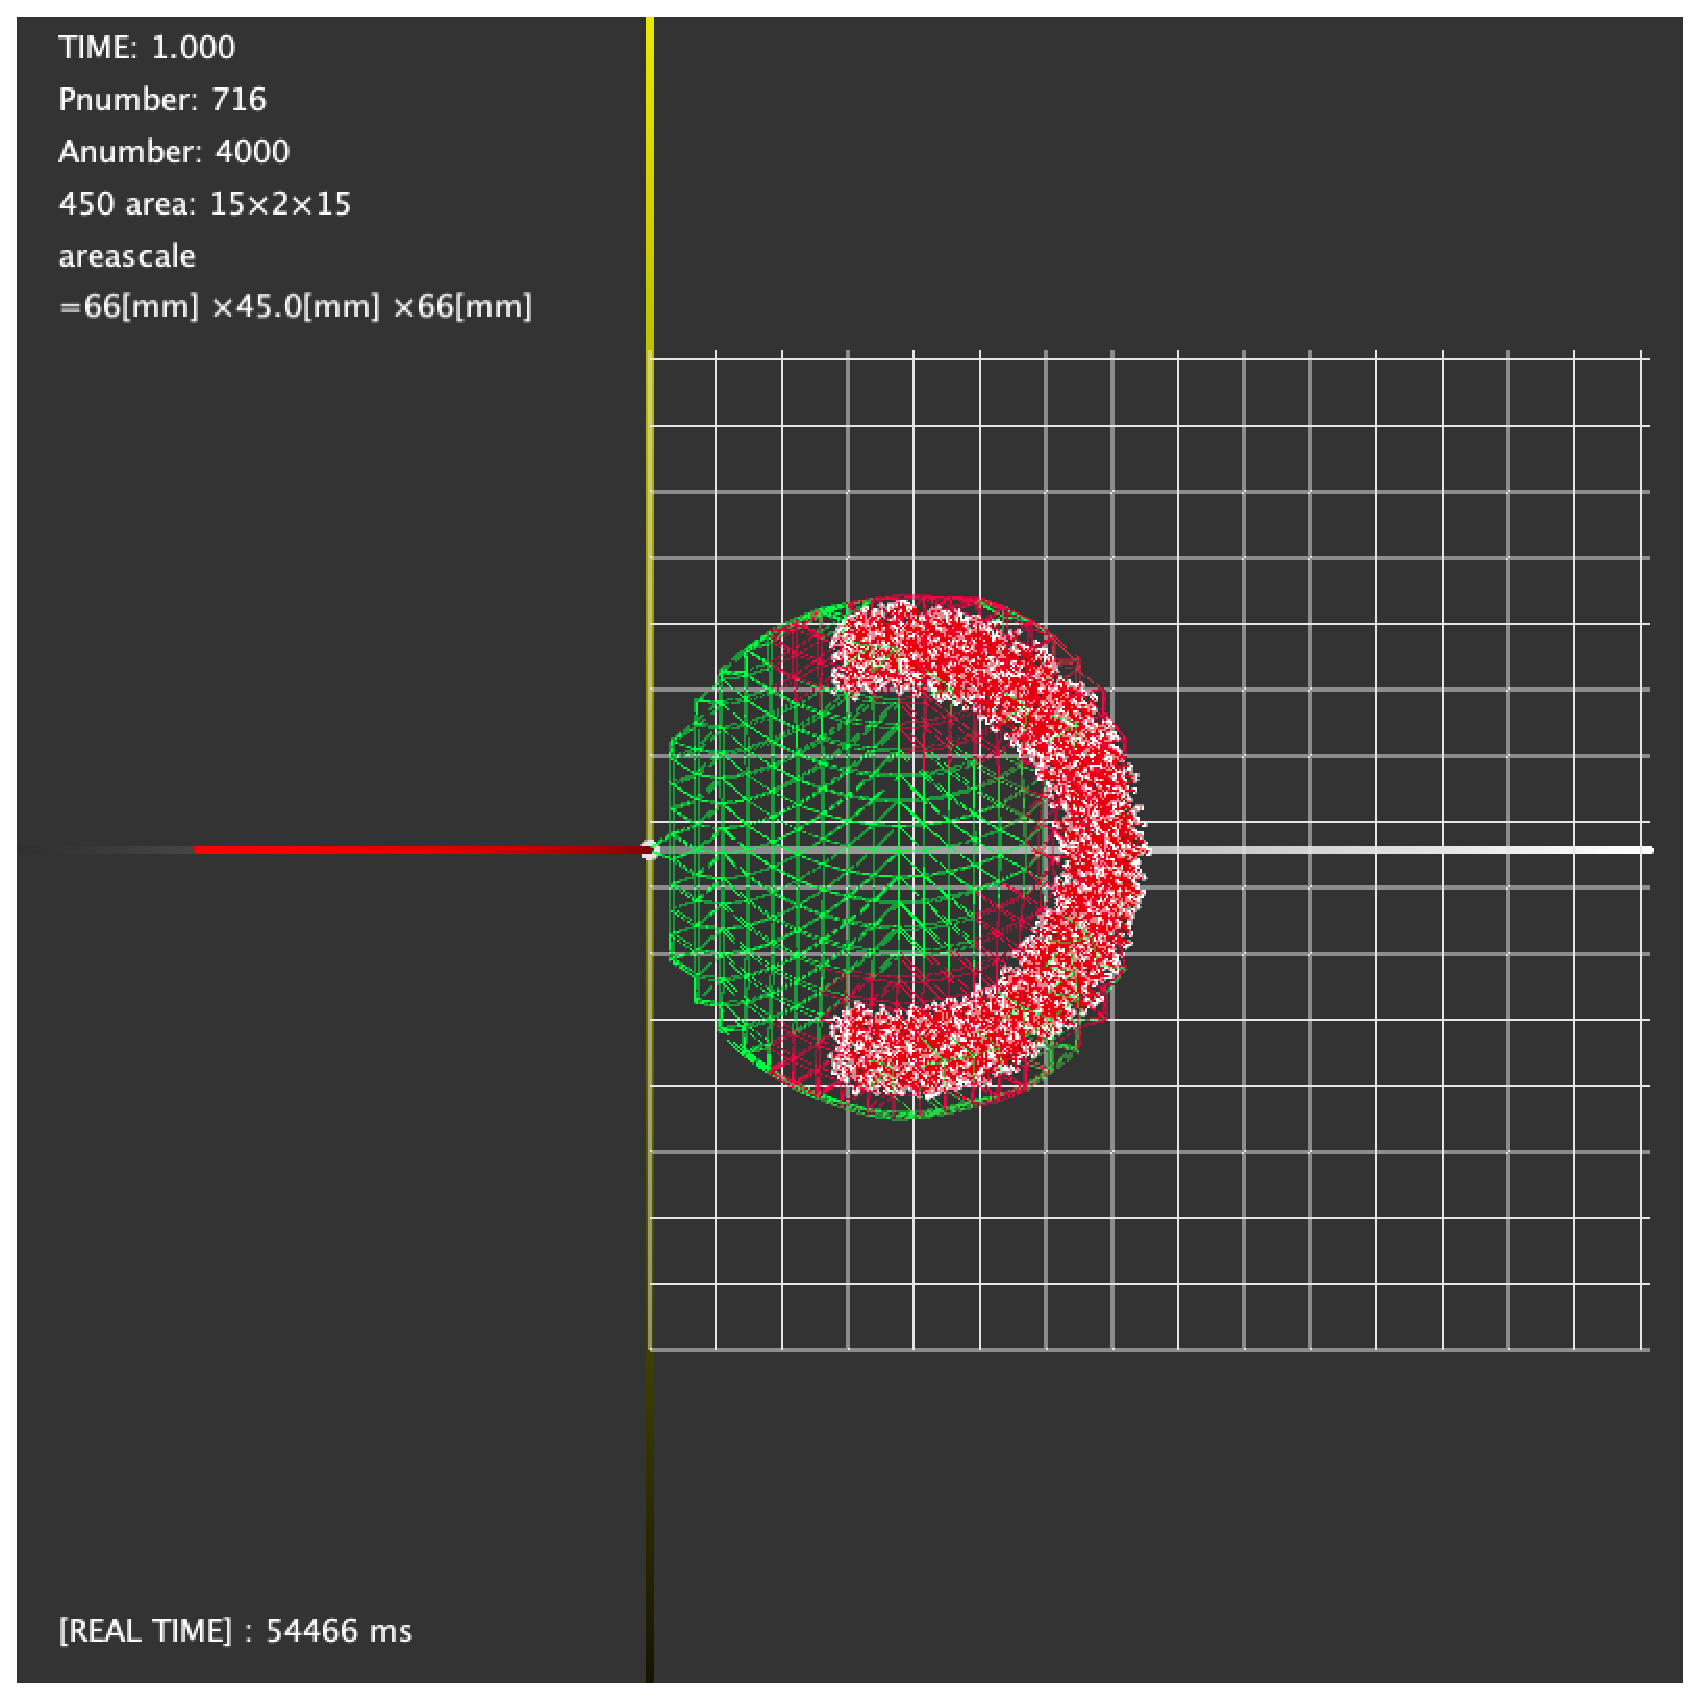
\includegraphics[width=5cm]{top10_darf.eps} 
  \end{tabular}
 }%
 \subfloat[]{%
  \begin{tabular}{c}
   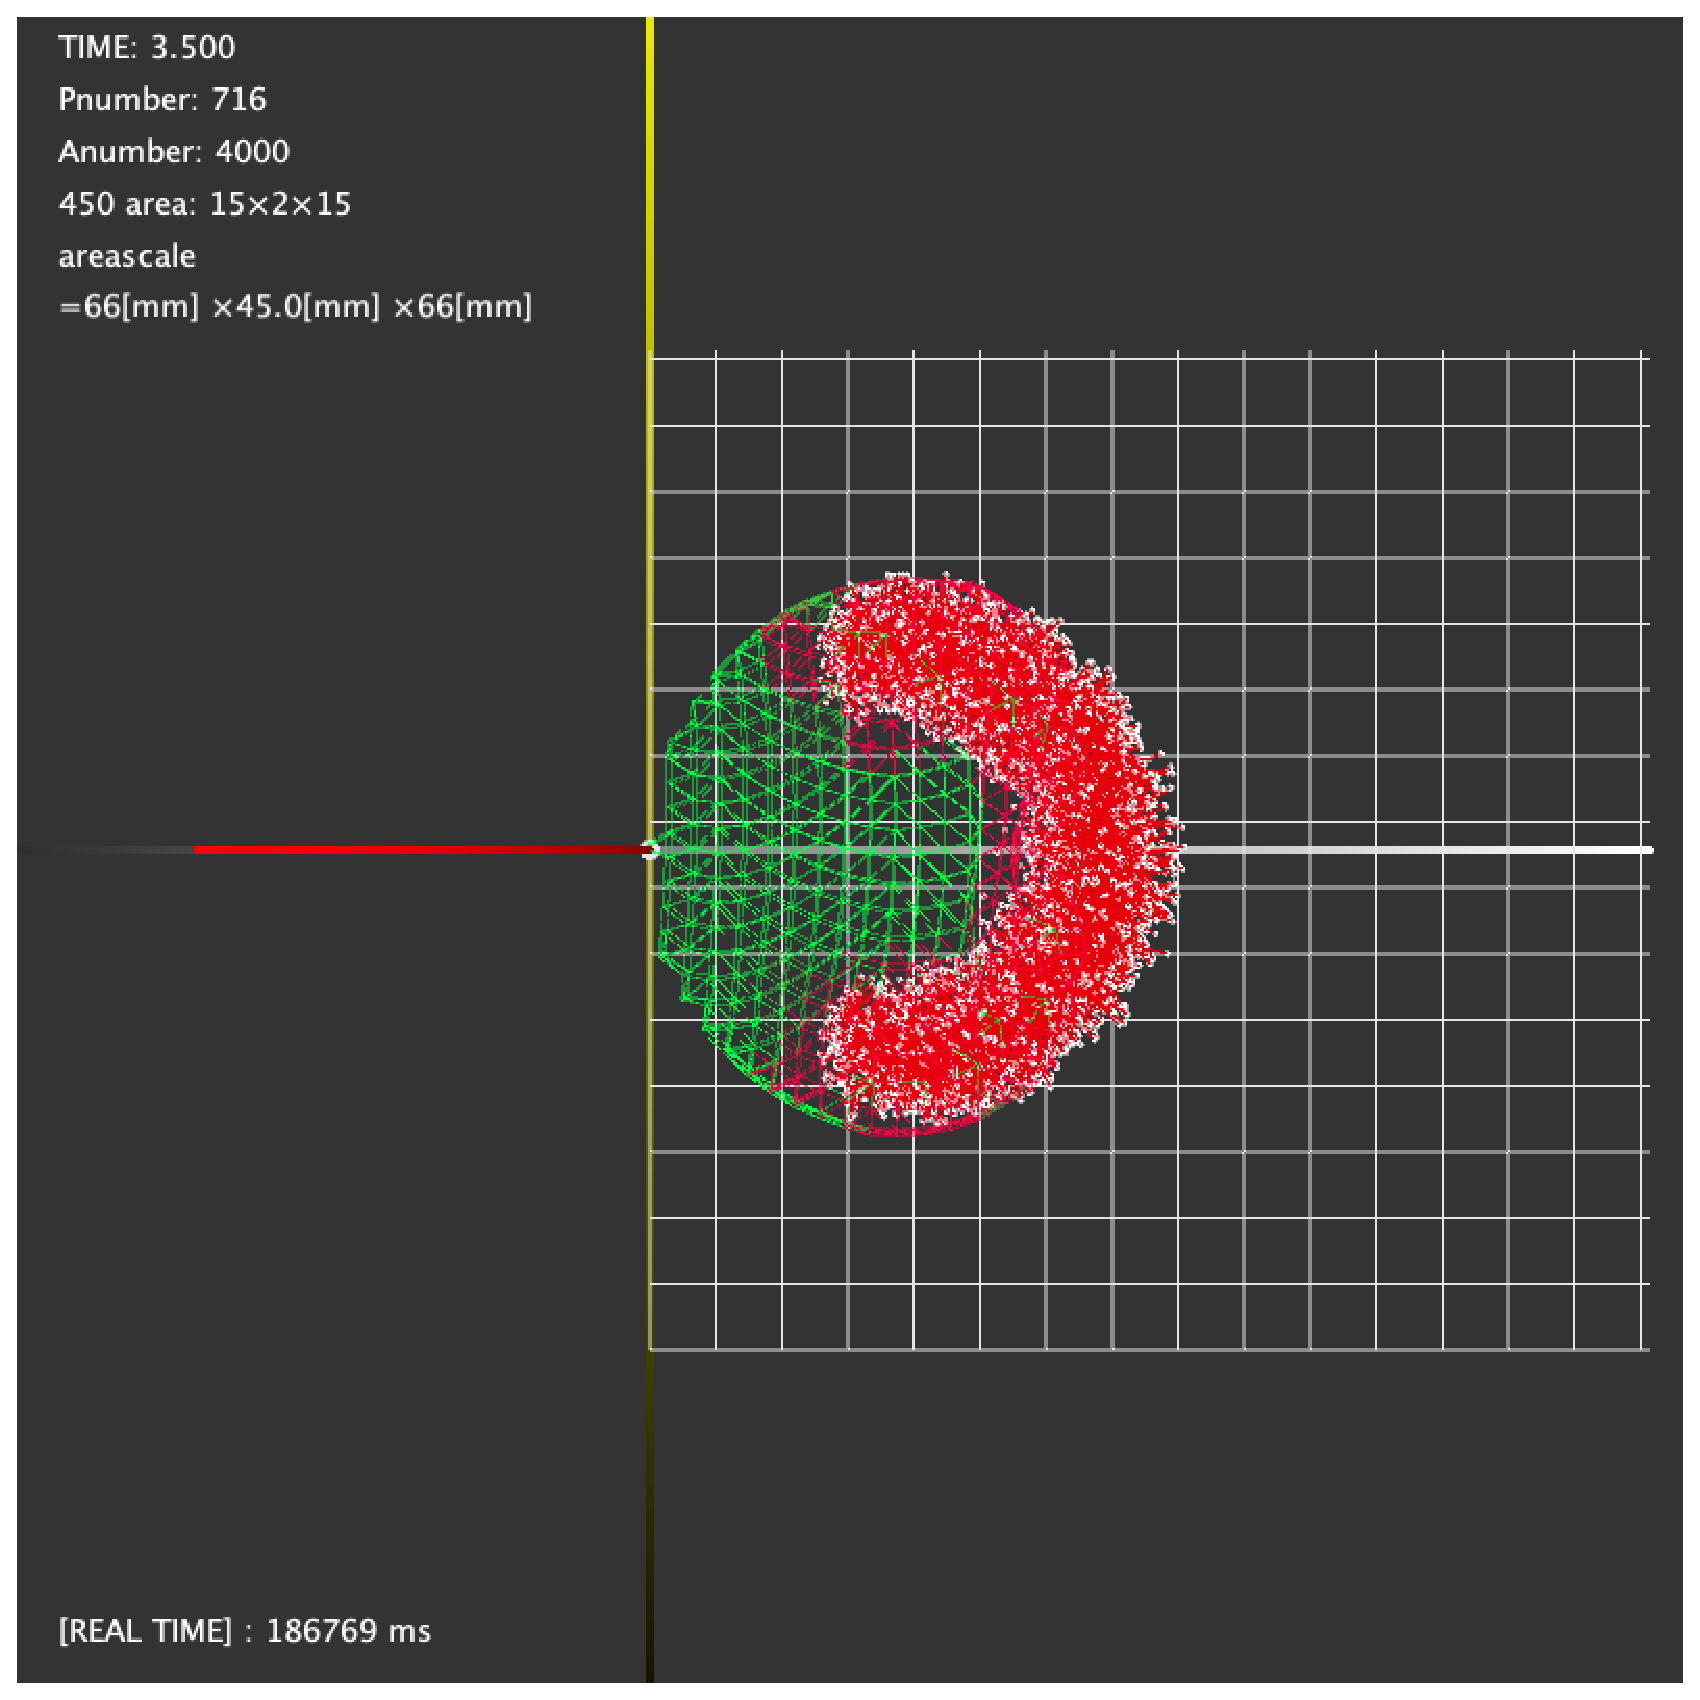
\includegraphics[width=5cm]{top35_darf.eps} 
  \end{tabular}
 }%
 \subfloat[]{%
  \begin{tabular}{c}
   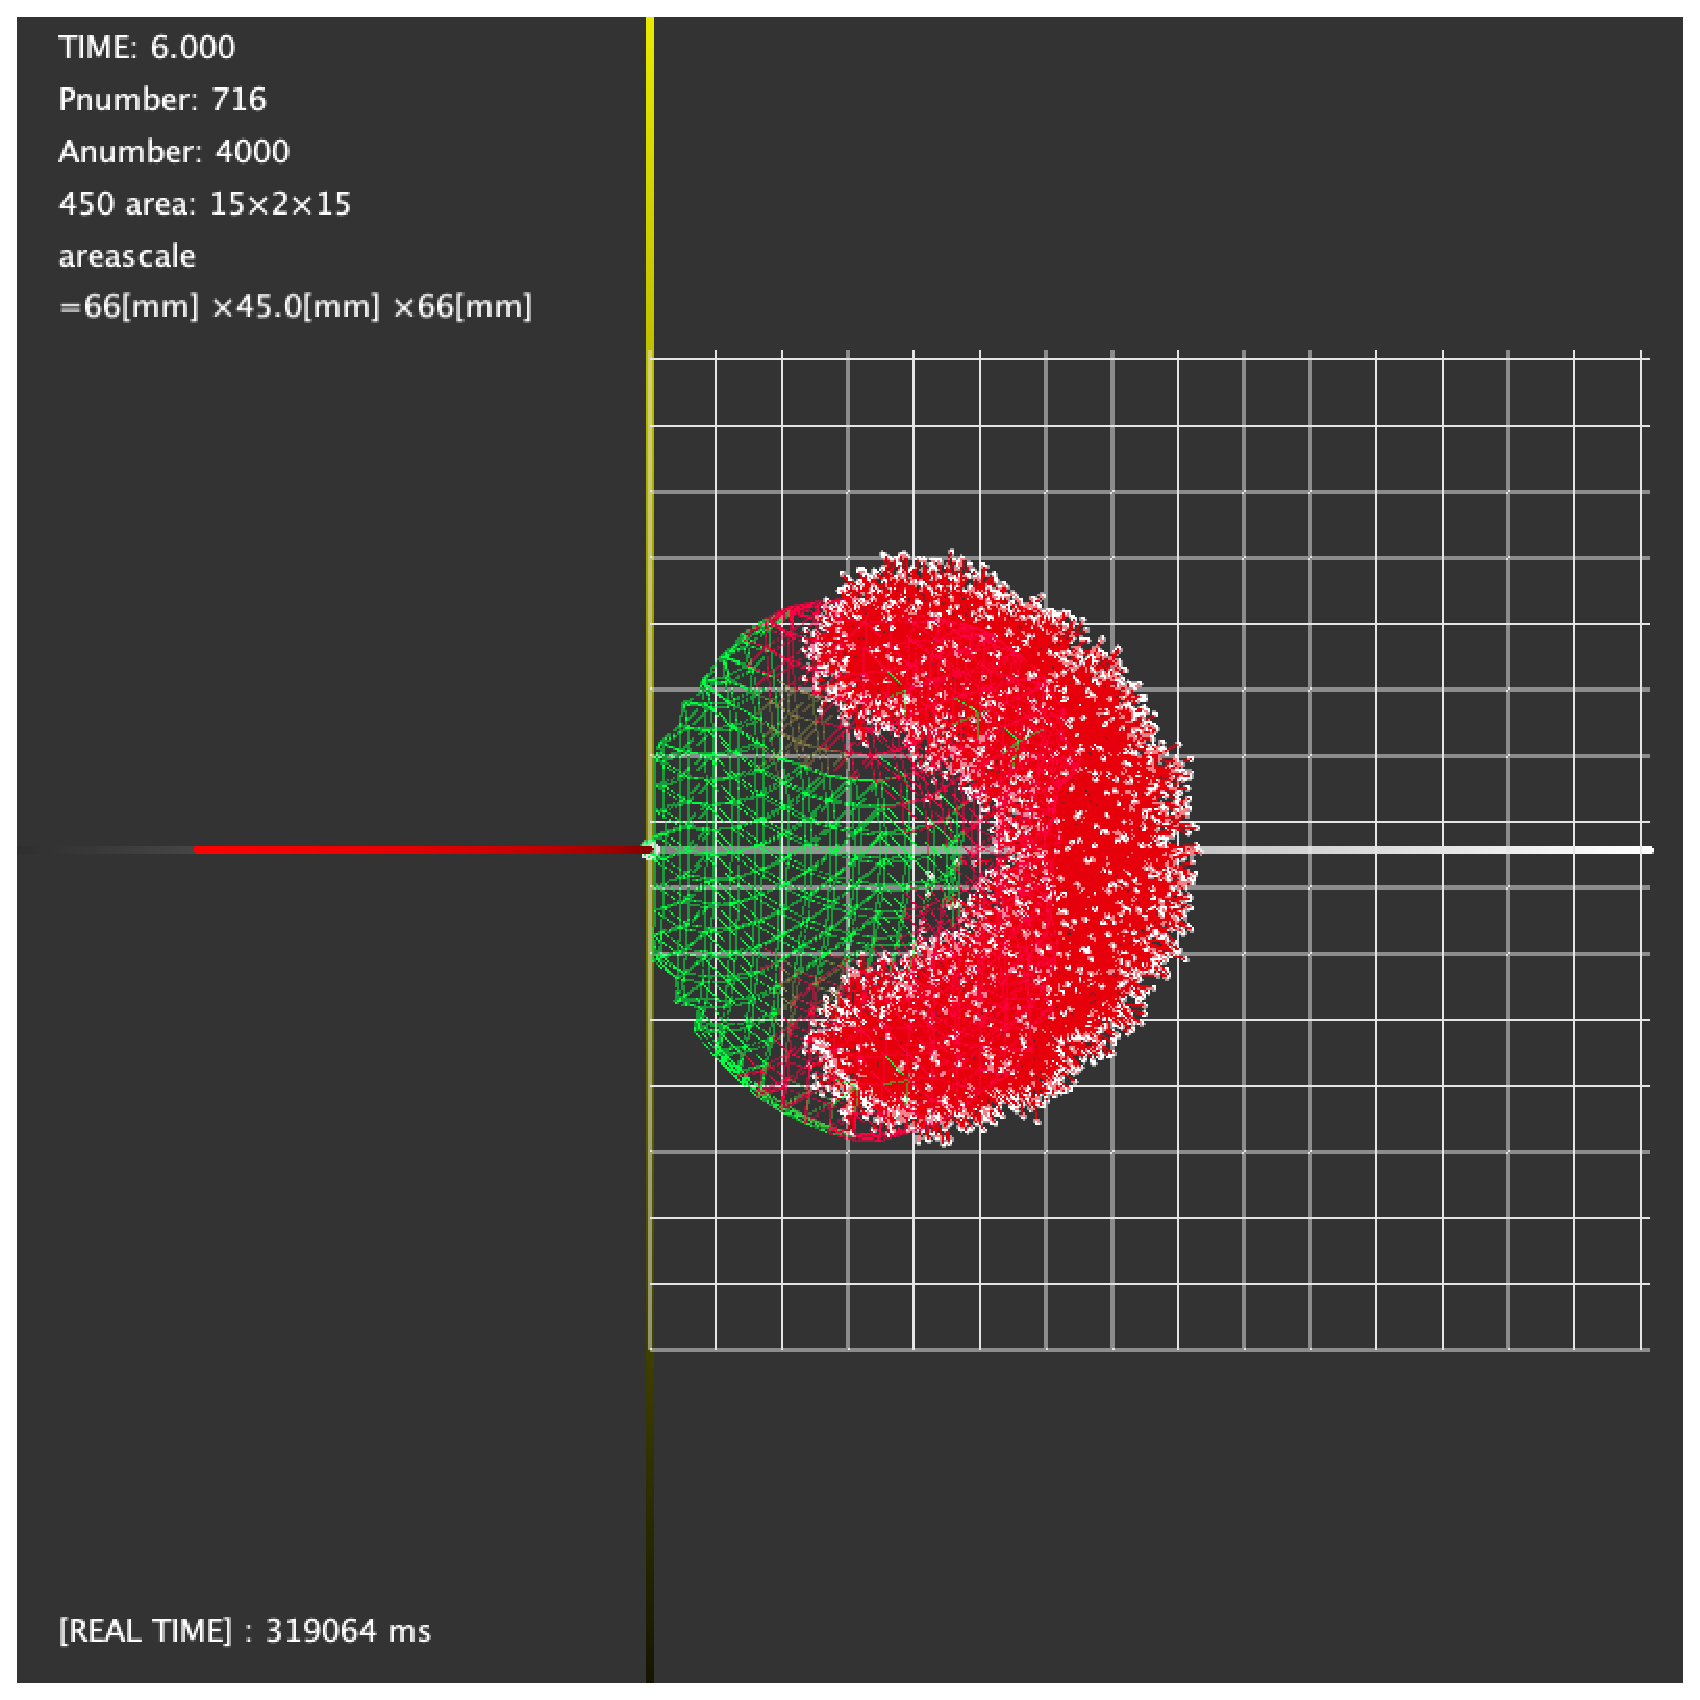
\includegraphics[width=5cm]{top60_darf.eps} 
  \end{tabular}
 }%
 \caption{A simulation result of ARF when $w = 2$ in Equation \ref{eq:arf}.}
 \label{fig:res1}
\end{figure}

%RP、距離非依存
\begin{figure}[tbp]
 \subfloat[]{%
  \begin{tabular}{c}
   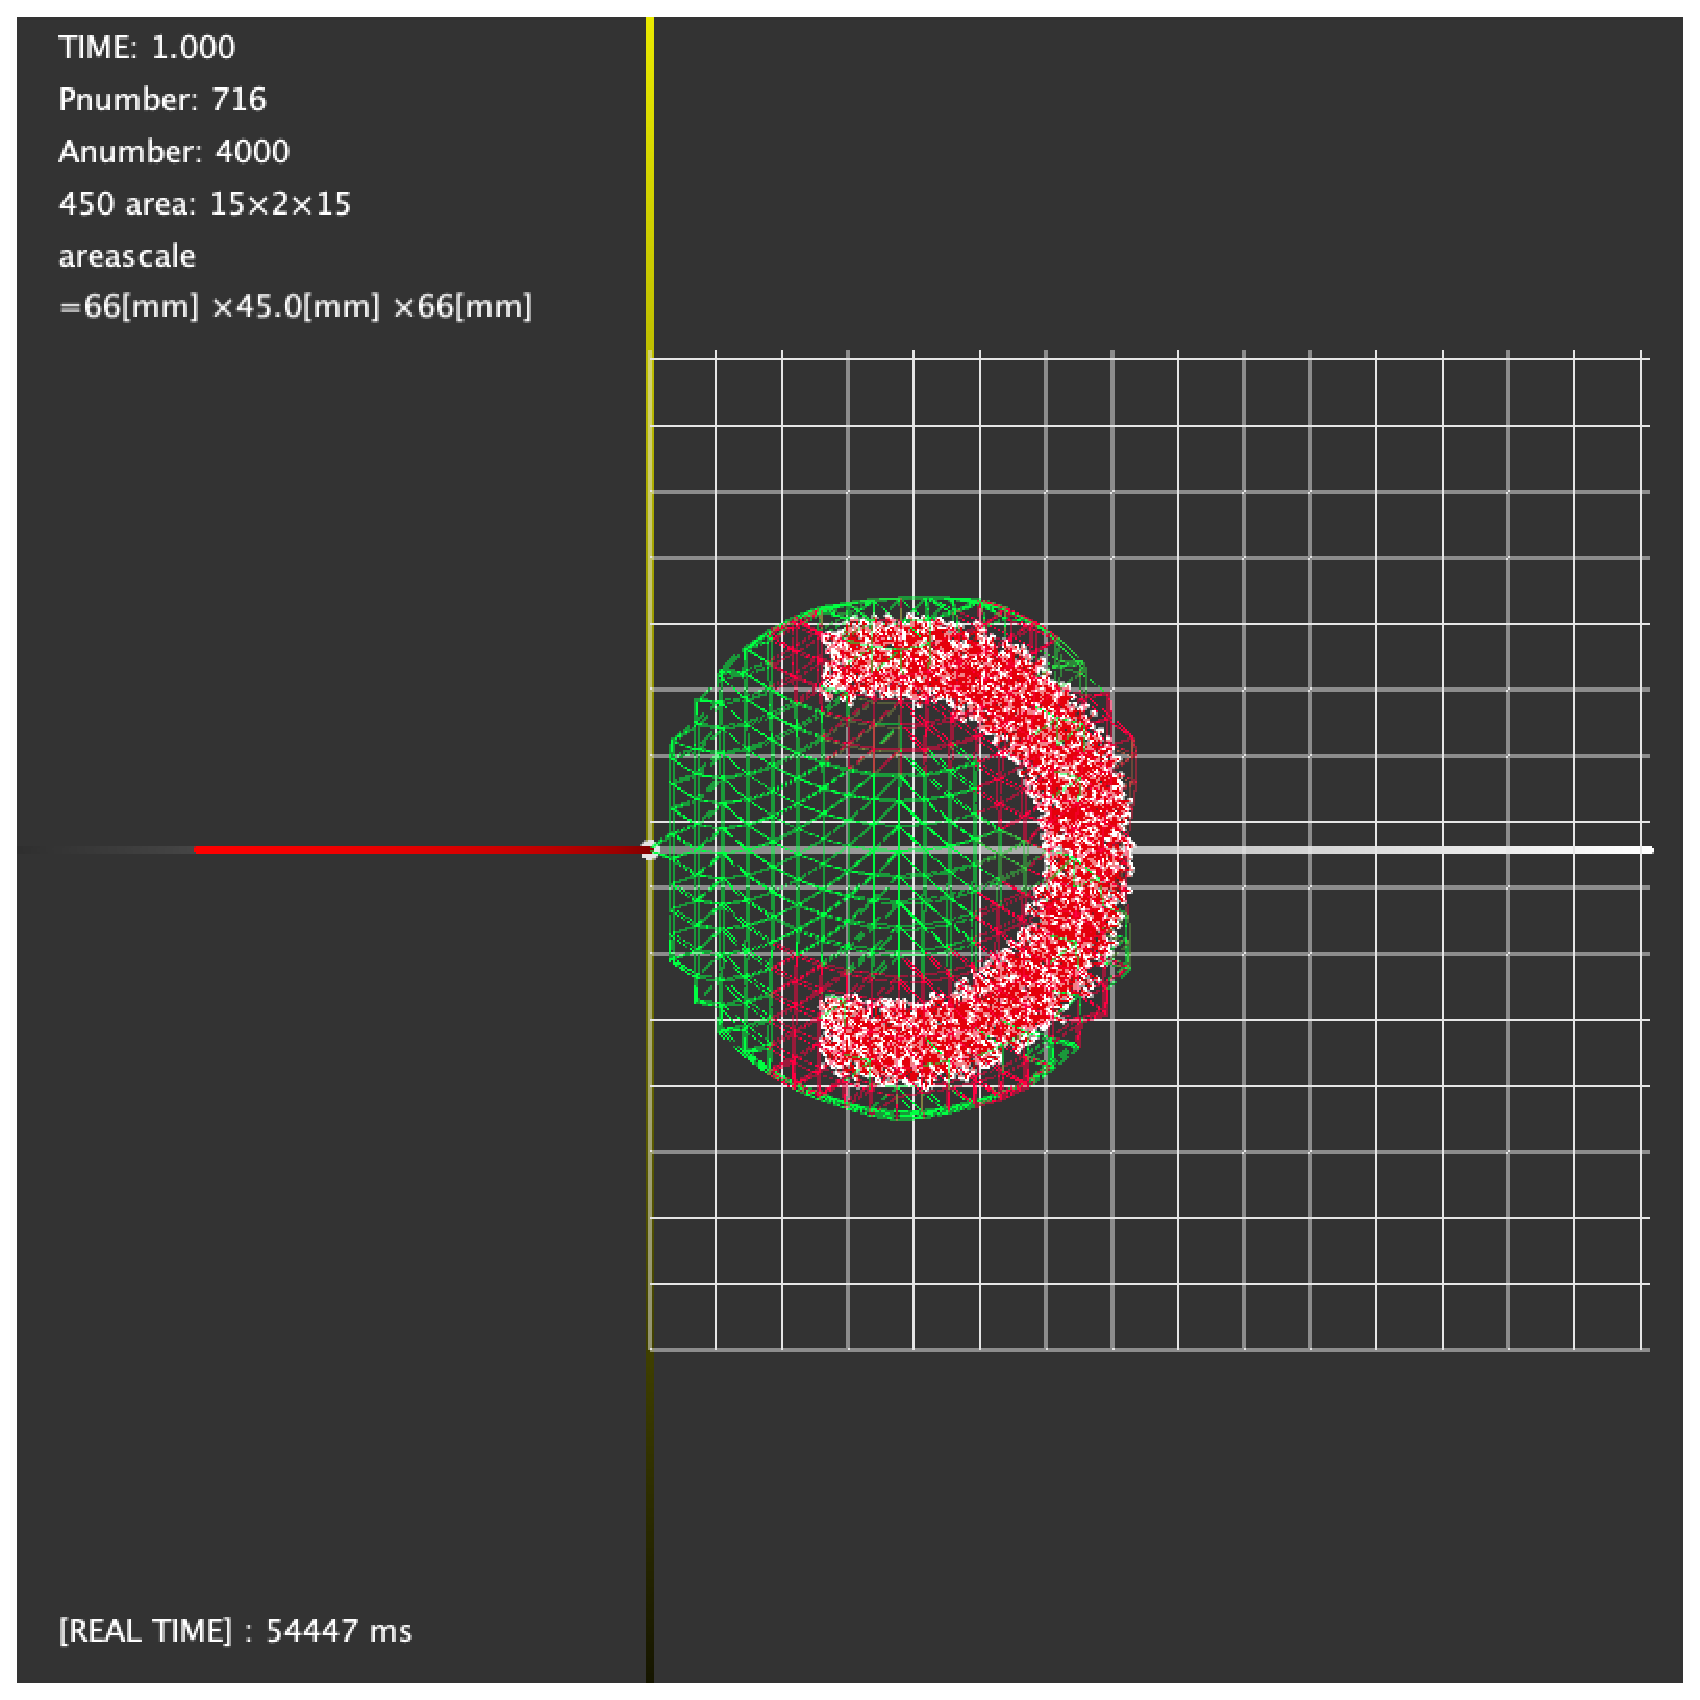
\includegraphics[width=5cm]{top10_1arf.eps} 
  \end{tabular}
 }%
 \subfloat[]{%
  \begin{tabular}{c}
   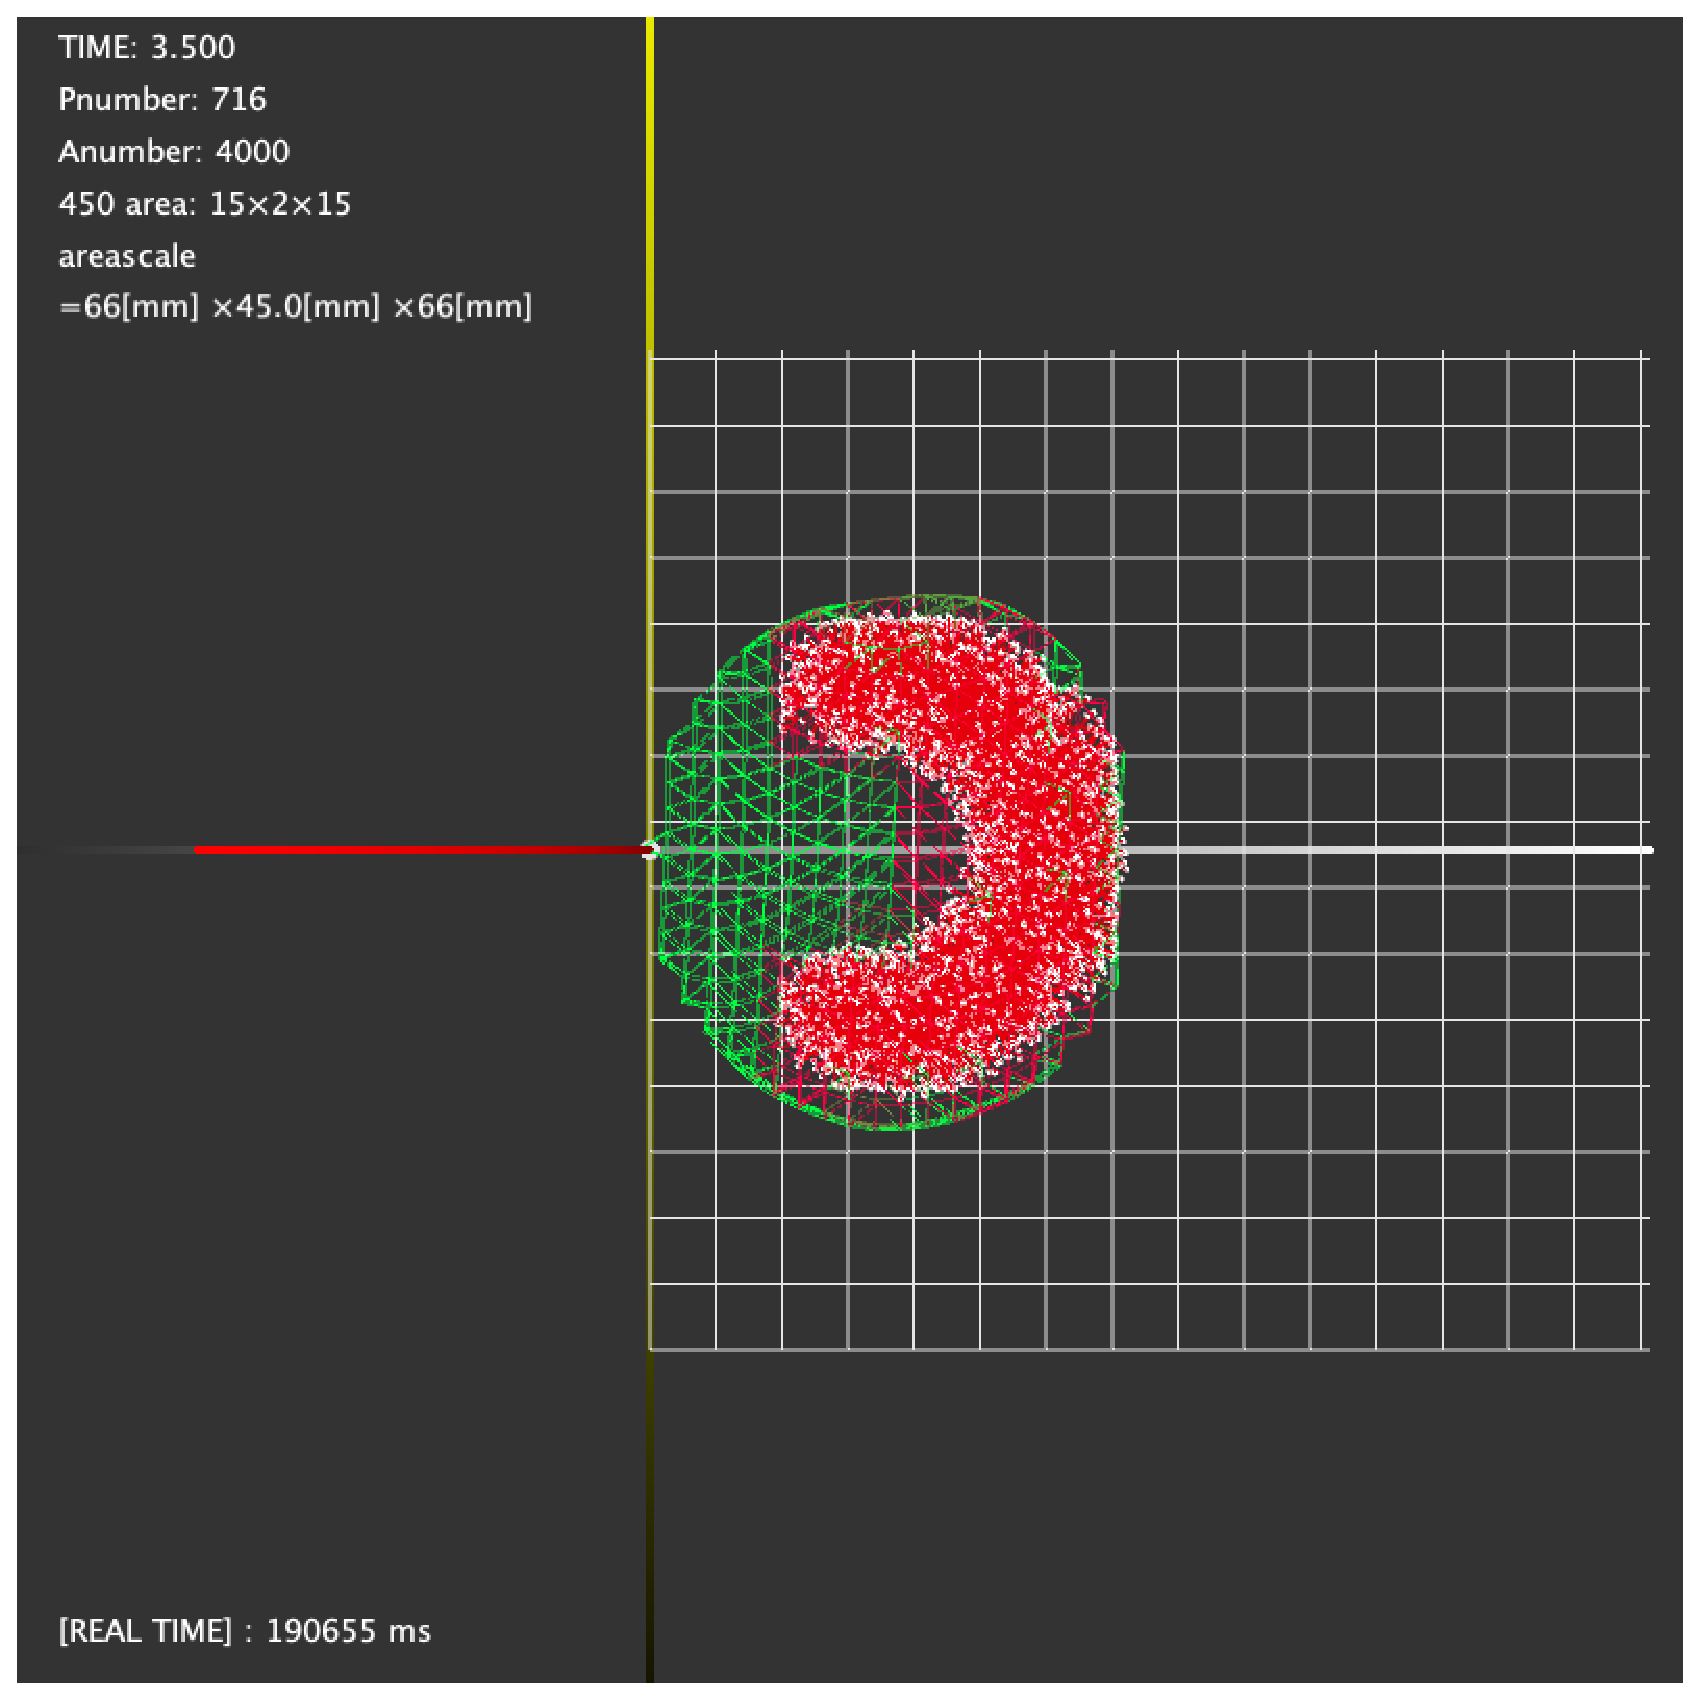
\includegraphics[width=5cm]{top35_1arf.eps}
  \end{tabular}
 }%
 \subfloat[]{%
  \begin{tabular}{c}
   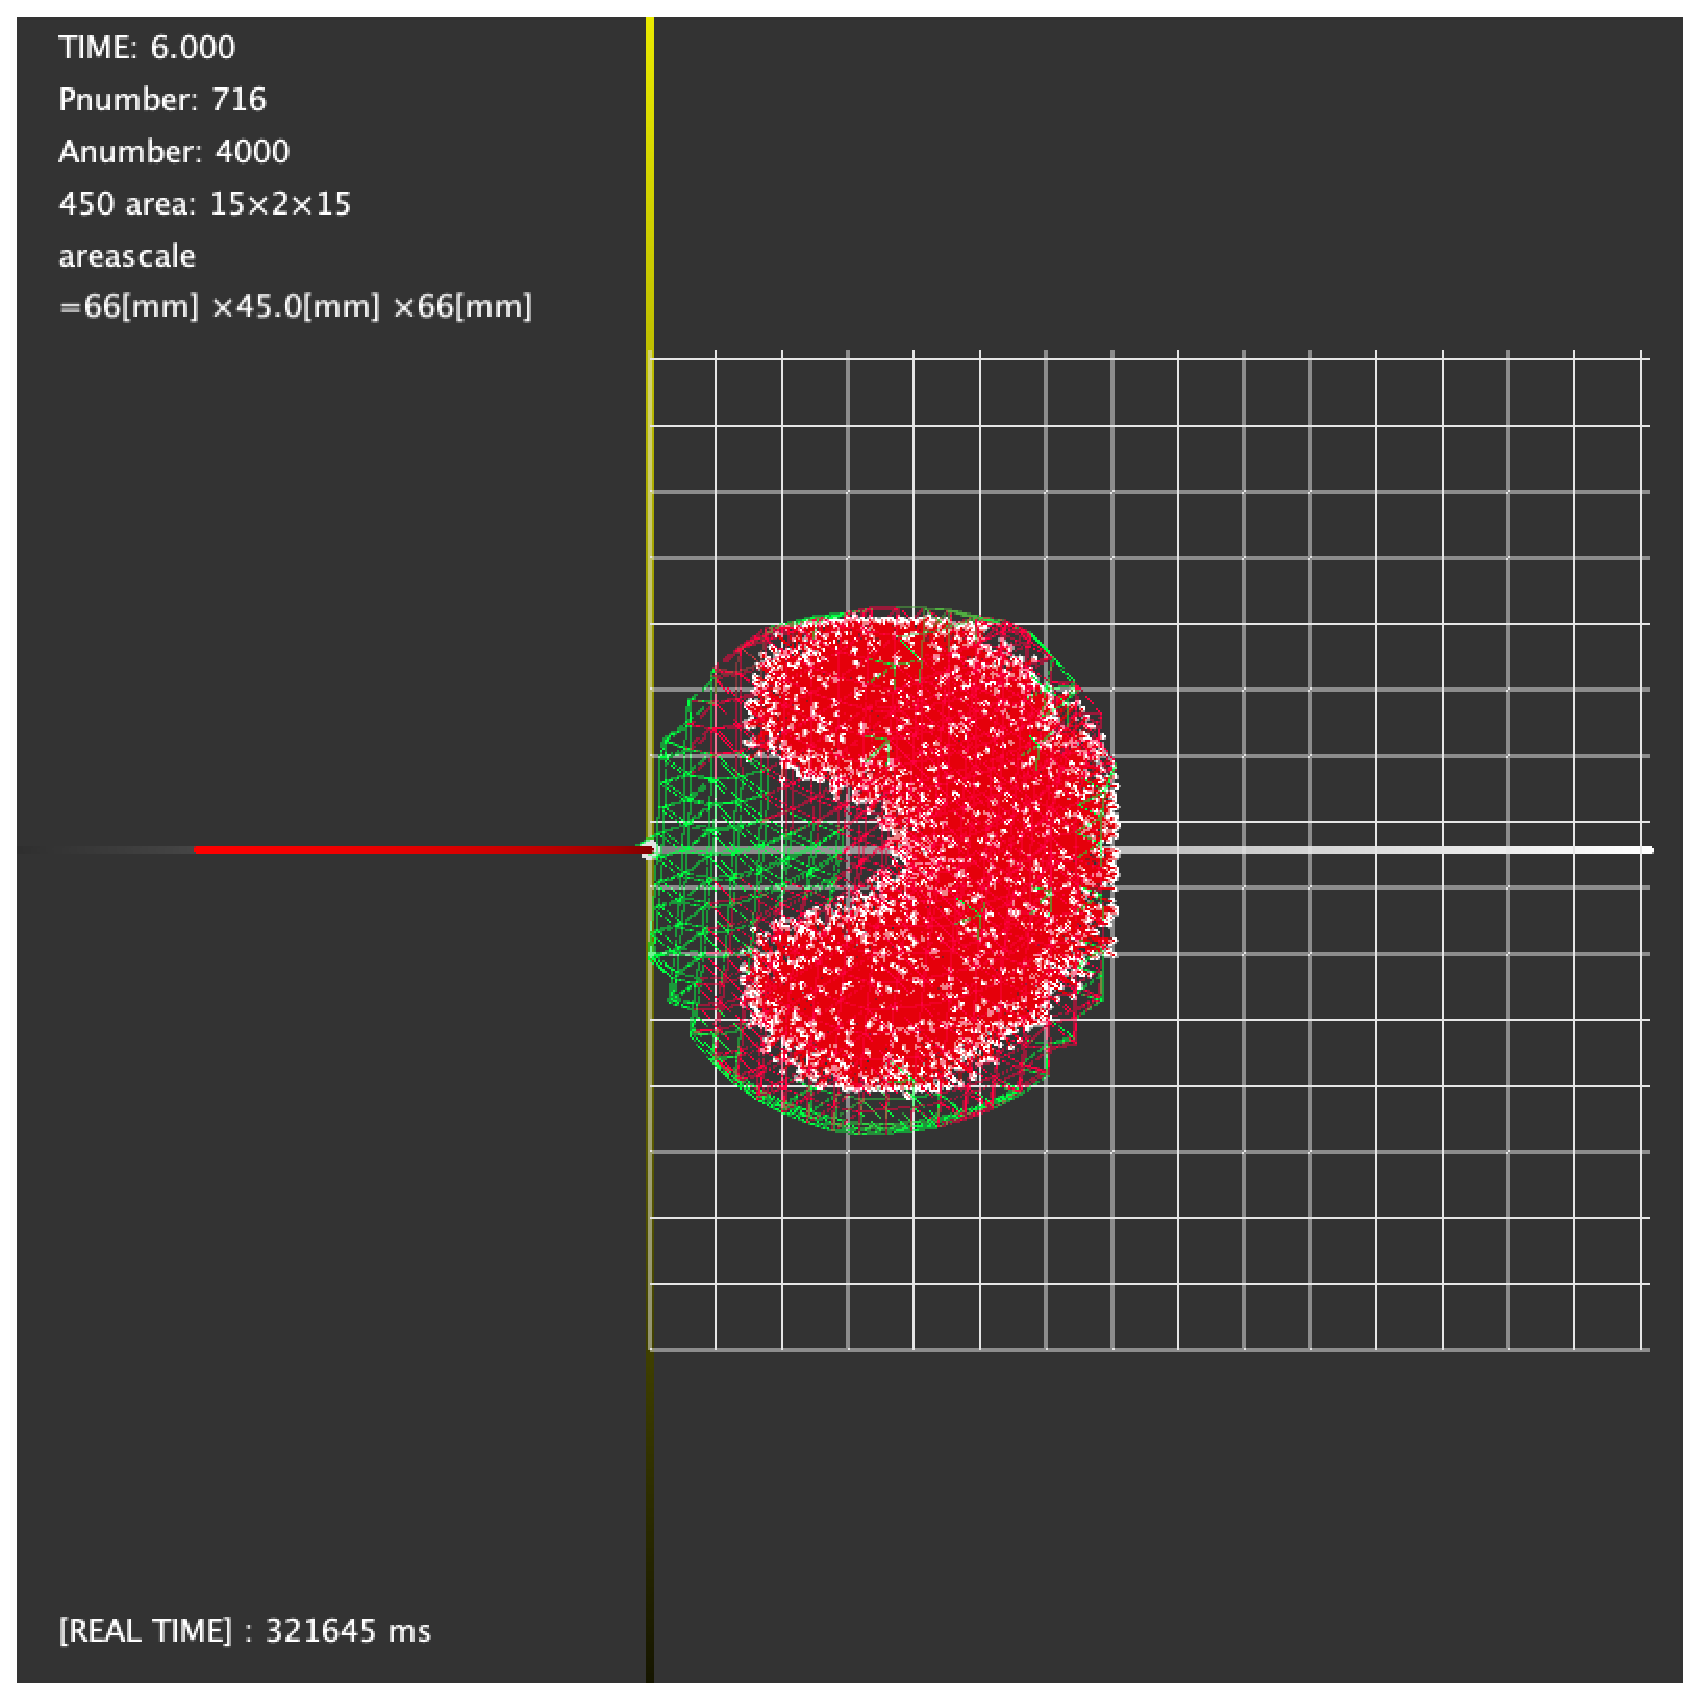
\includegraphics[width=5cm]{top60_1arf.eps} 
  \end{tabular}
 }%
 \caption{Simulation results when the reference point of the ARF is assumed as the leftmost membrane molecule of the cell.}
 \label{fig:res2}
\end{figure}

%NON ARF

\begin{figure}[tbp]
 \subfloat[]{%
  \begin{tabular}{c}
   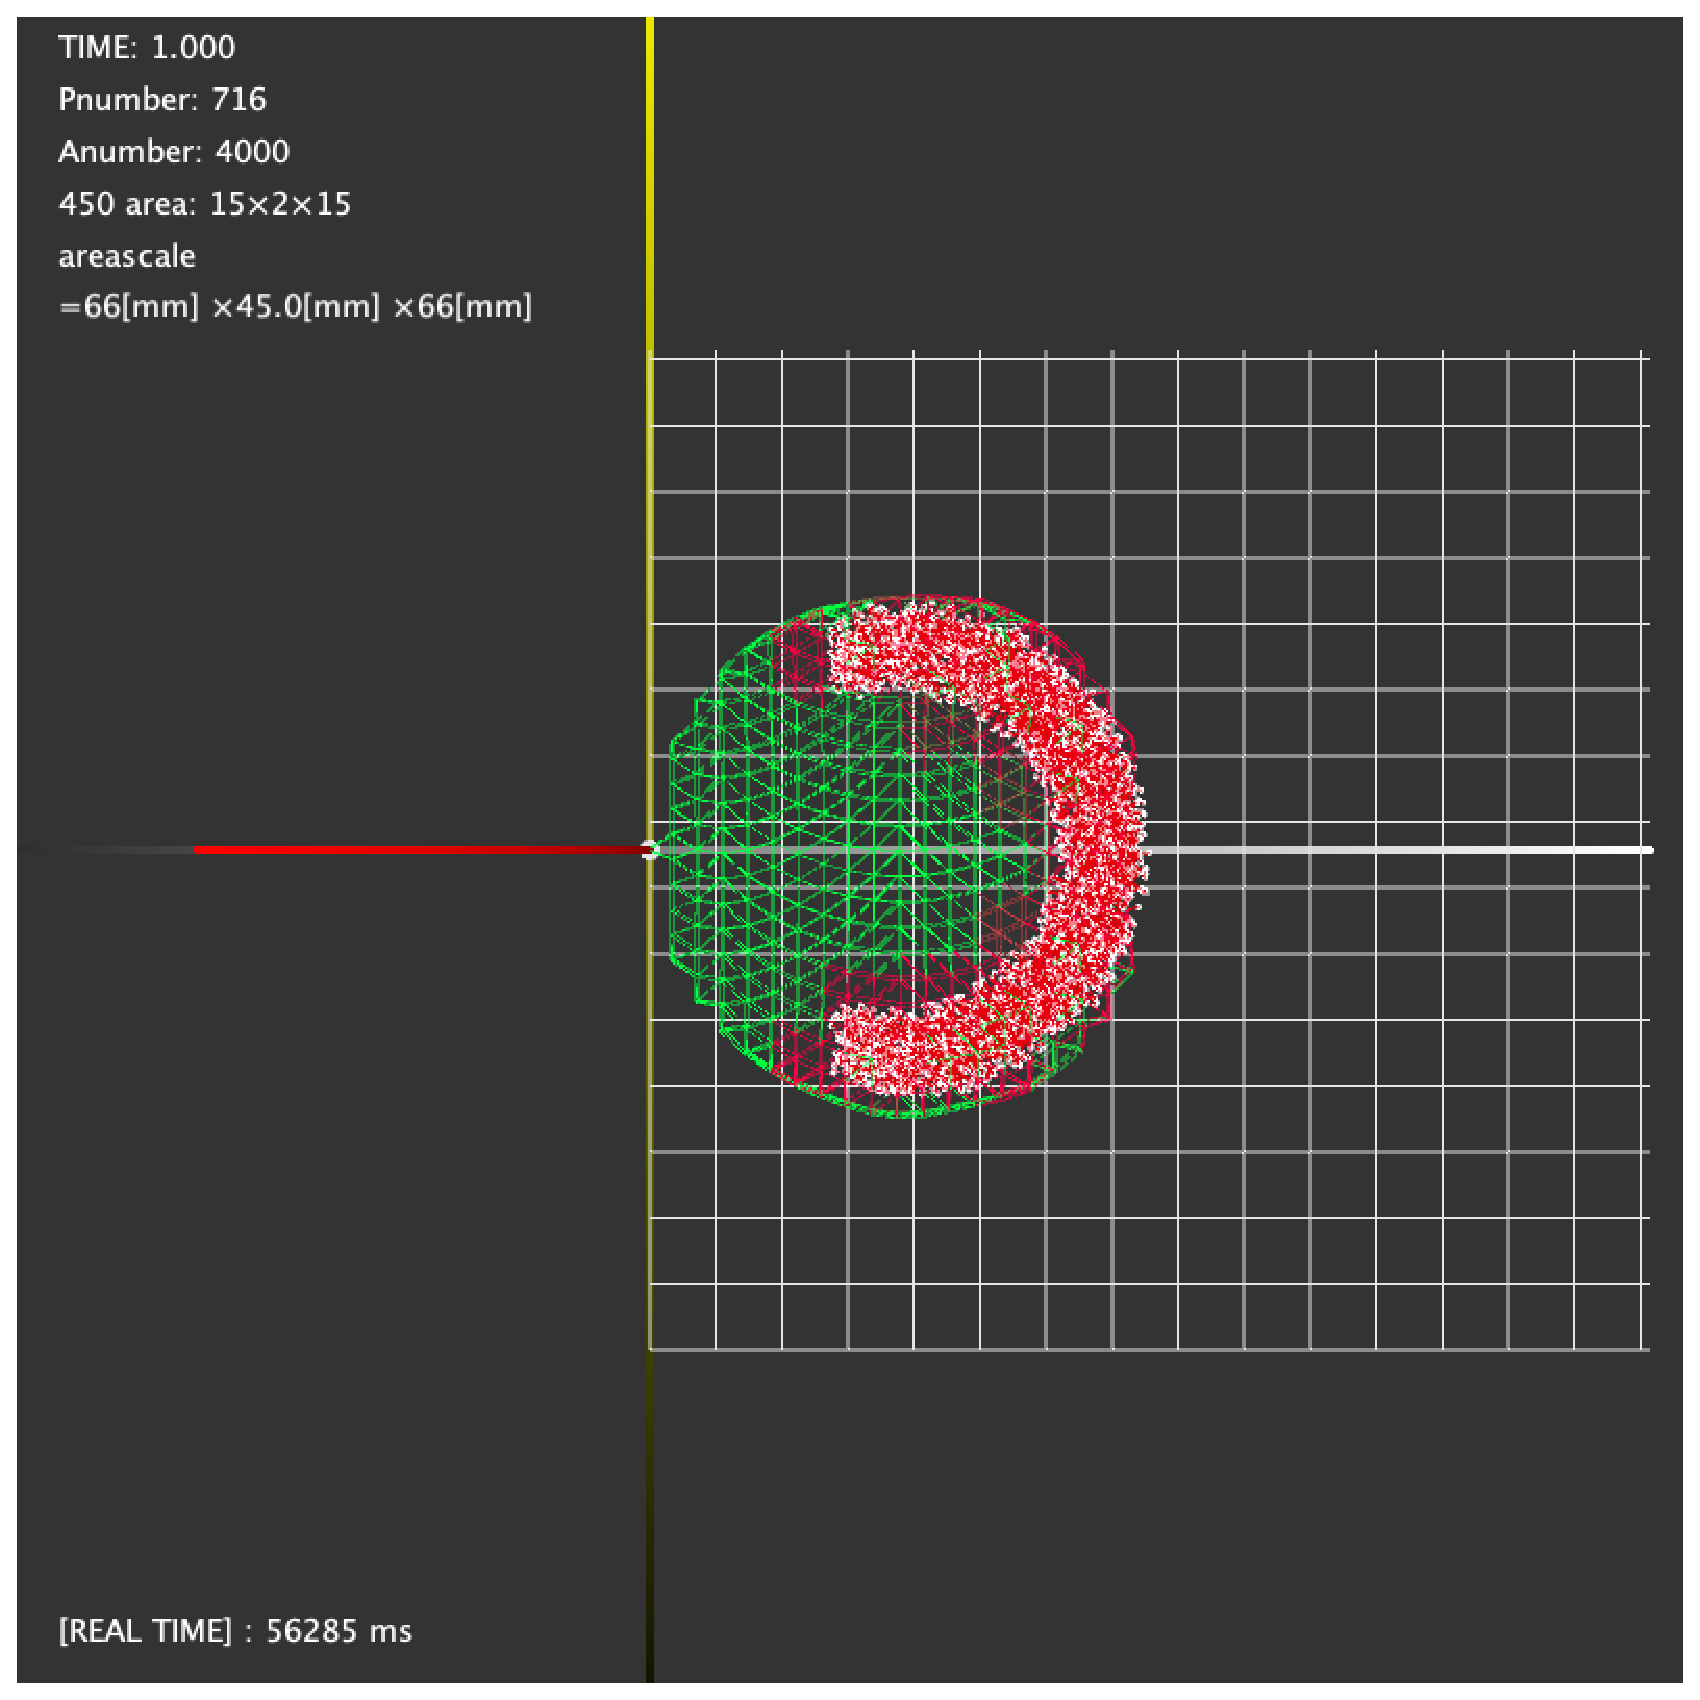
\includegraphics[width=5cm]{top10_narf.eps} 
  \end{tabular}
 }%
 \subfloat[]{%
  \begin{tabular}{c}
   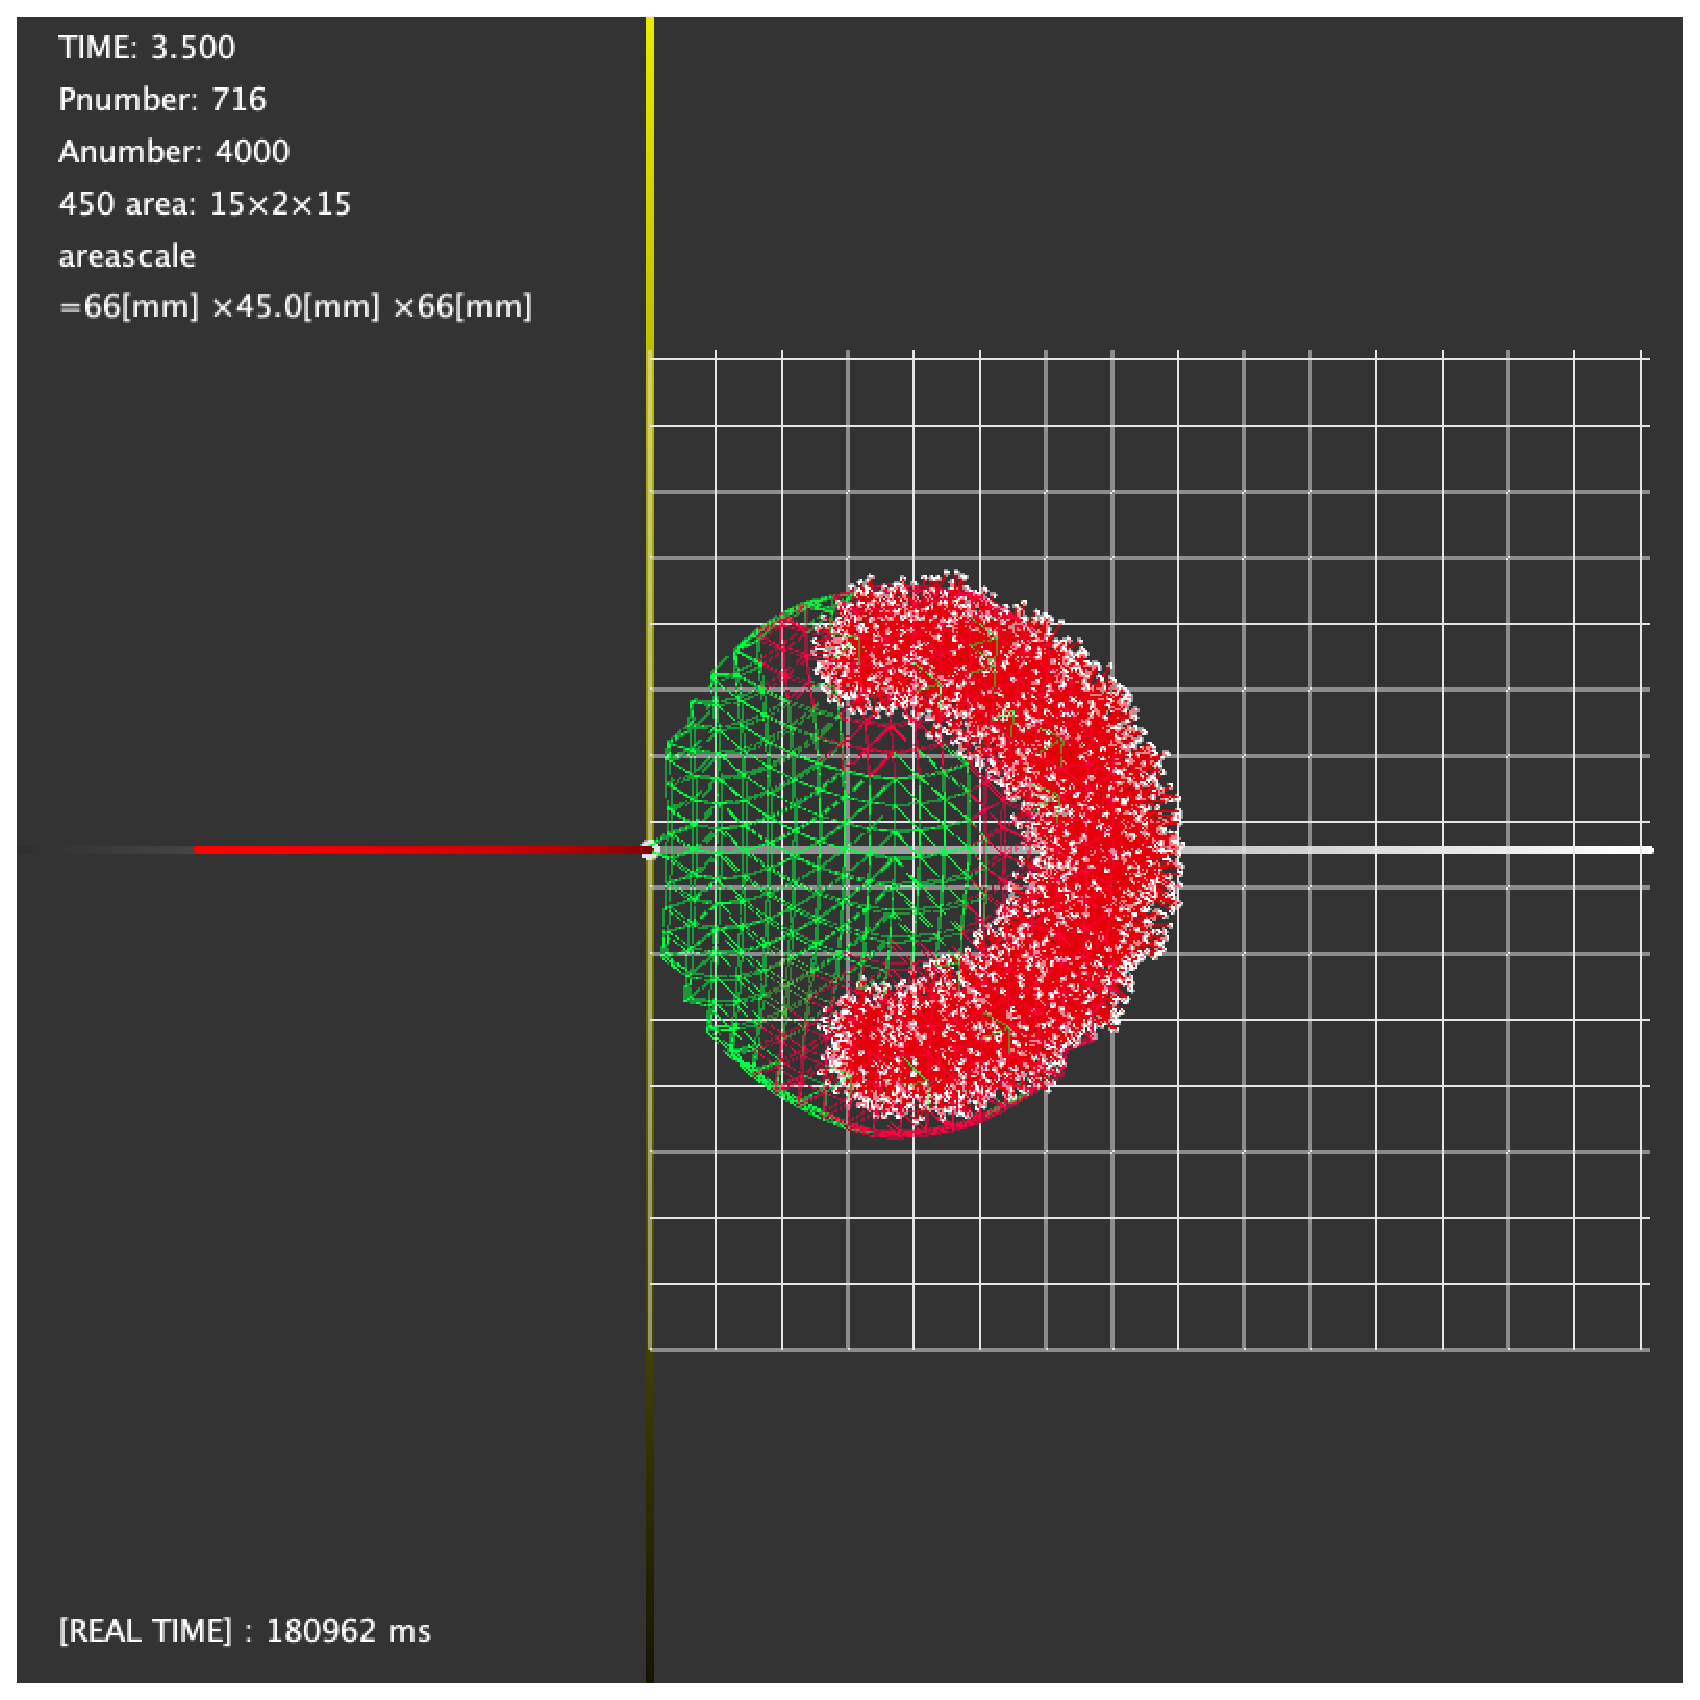
\includegraphics[width=5cm]{top35_narf.eps}
  \end{tabular}
 }%
 \subfloat[]{%
  \begin{tabular}{c}
   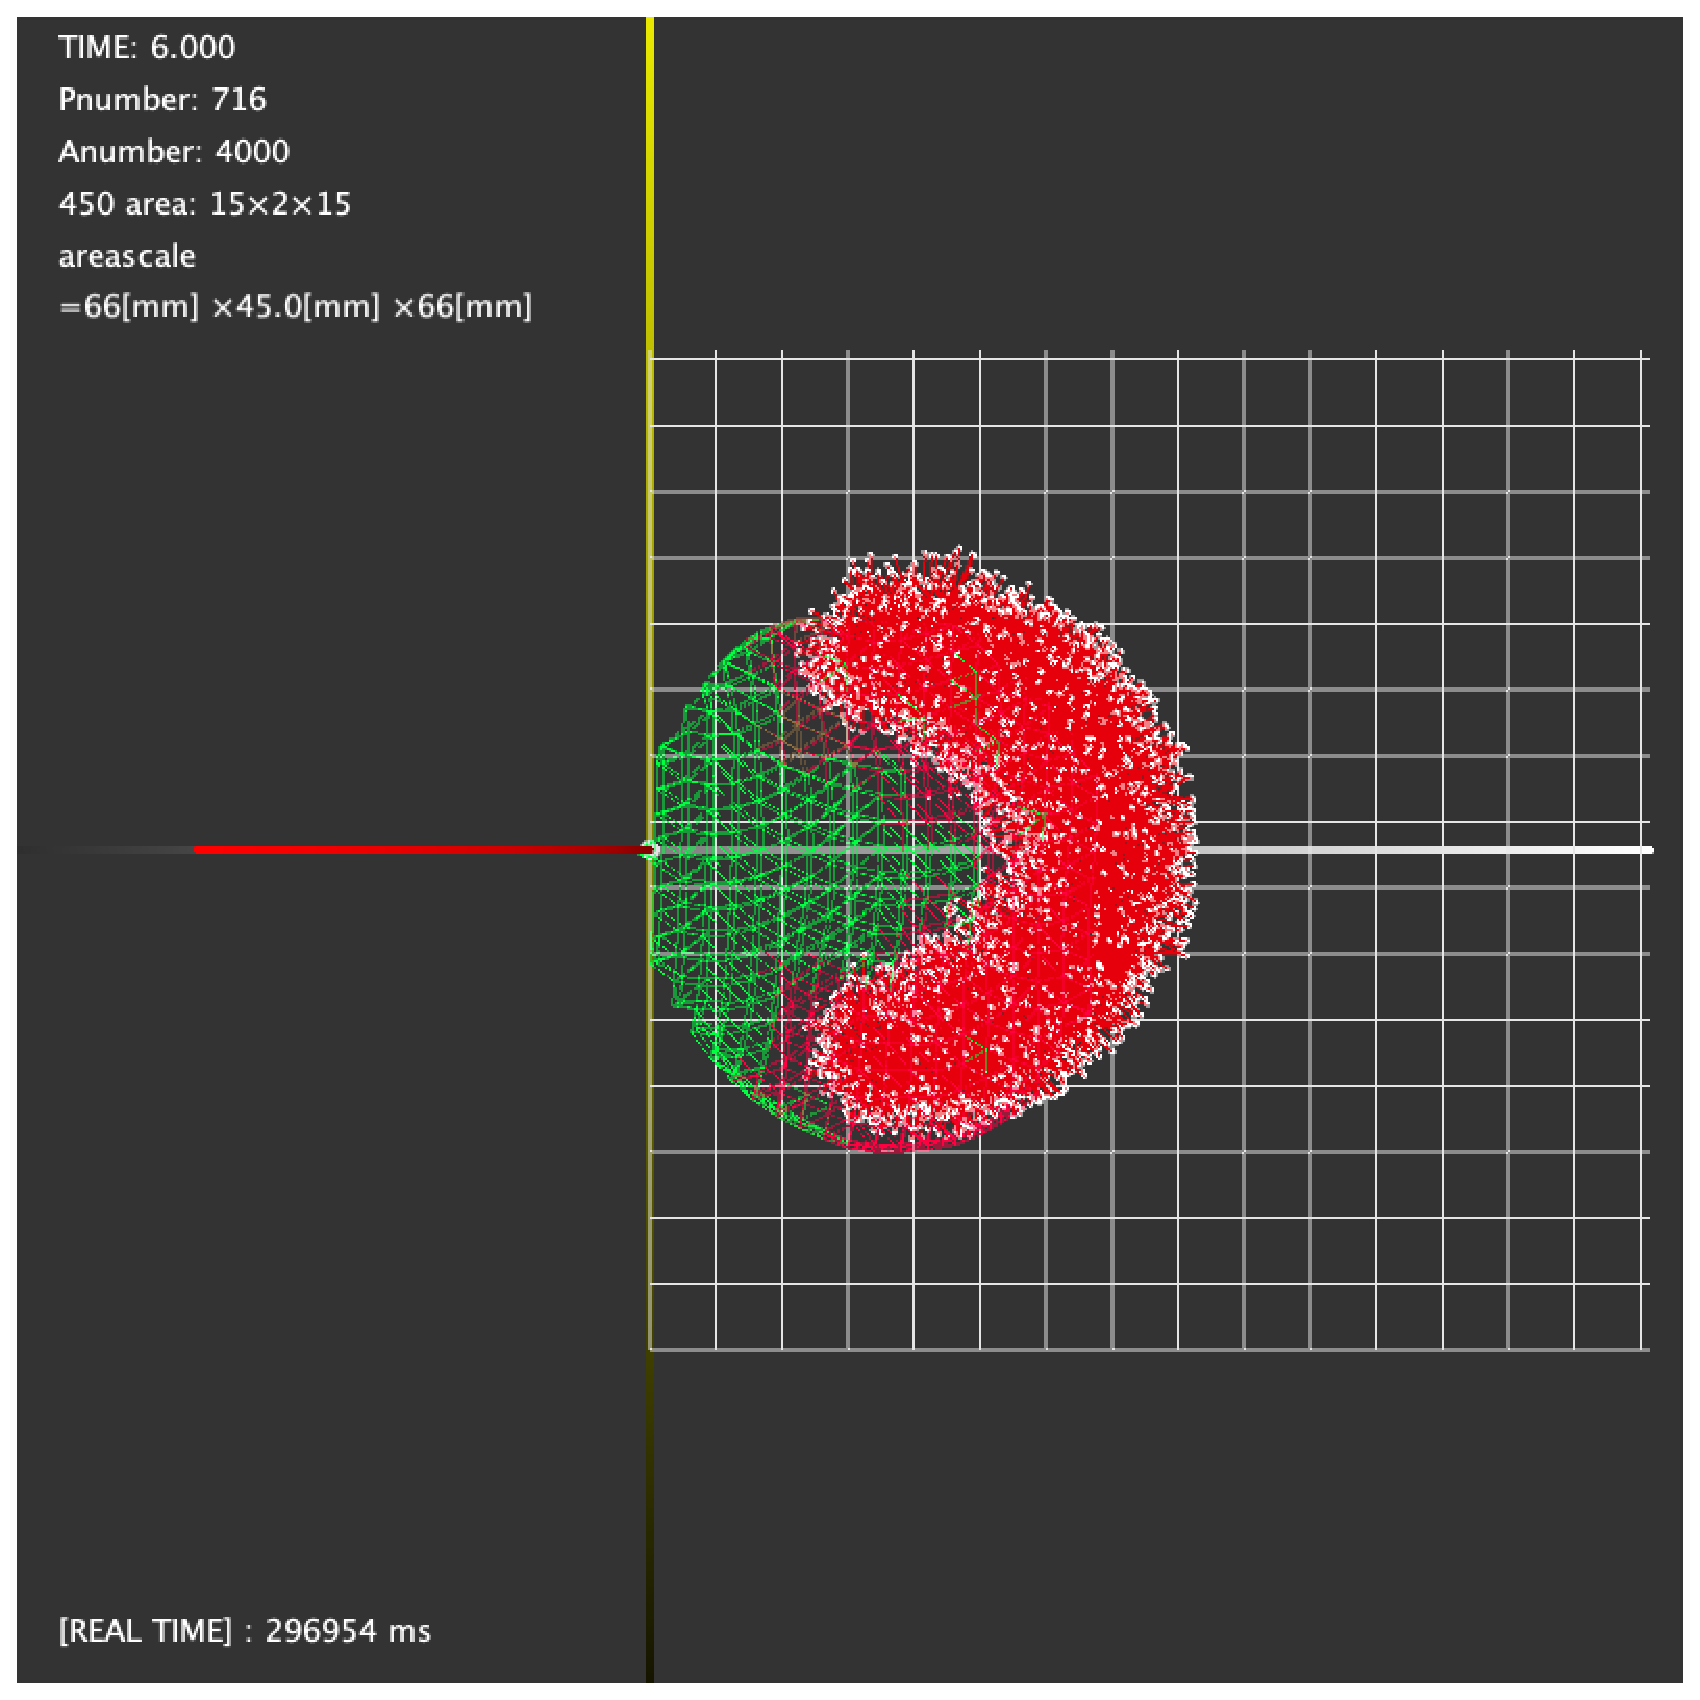
\includegraphics[width=5cm]{top60_narf.eps} 
  \end{tabular}
 }%
 \caption{Simulation Results without ARF.}
 \label{fig:res3}
\end{figure}

Fig. \ref{fig:res0} showed the simulation result when two reference points of the ARF were prepared (eq. \ref{eq:arf}) and the effect of the ARF was independent of the distance (w=1).
In this case, the actin molecule aggregated in a half-moon shape.
Fig.\ref{fig:res1} showed the simulation results under the same condition as Fig. \ref{fig:res0} except that distance-dependent ARF was  used (w=2).
In Fig. \ref{fig:res0}, the actin molecule protruded from the cell membrane as a result of continuing AP.
Fig.\ref{fig:res2} showed simulation results assuming that the ARF reference point is the last cell membrane molecule, not SF.
Deformation occurred towards the center of the cell rather than pulling at two points.
Fig.\ref{fig:res3} showed the simulation results when the effect of the ARF was ignored.
The actin molecule protruded from the cell membrane as in the case of Fig. \ref{fig:res1}.
From the experimental results, the conditions under which the actin molecule is most stable are the conditions shown in Fig. \ref{fig:res0}.


\subsection{Effect of Initial Distribution of Actin Molecules}

\begin{figure}[tbp]
 \subfloat[]{%
  \begin{tabular}{c}
   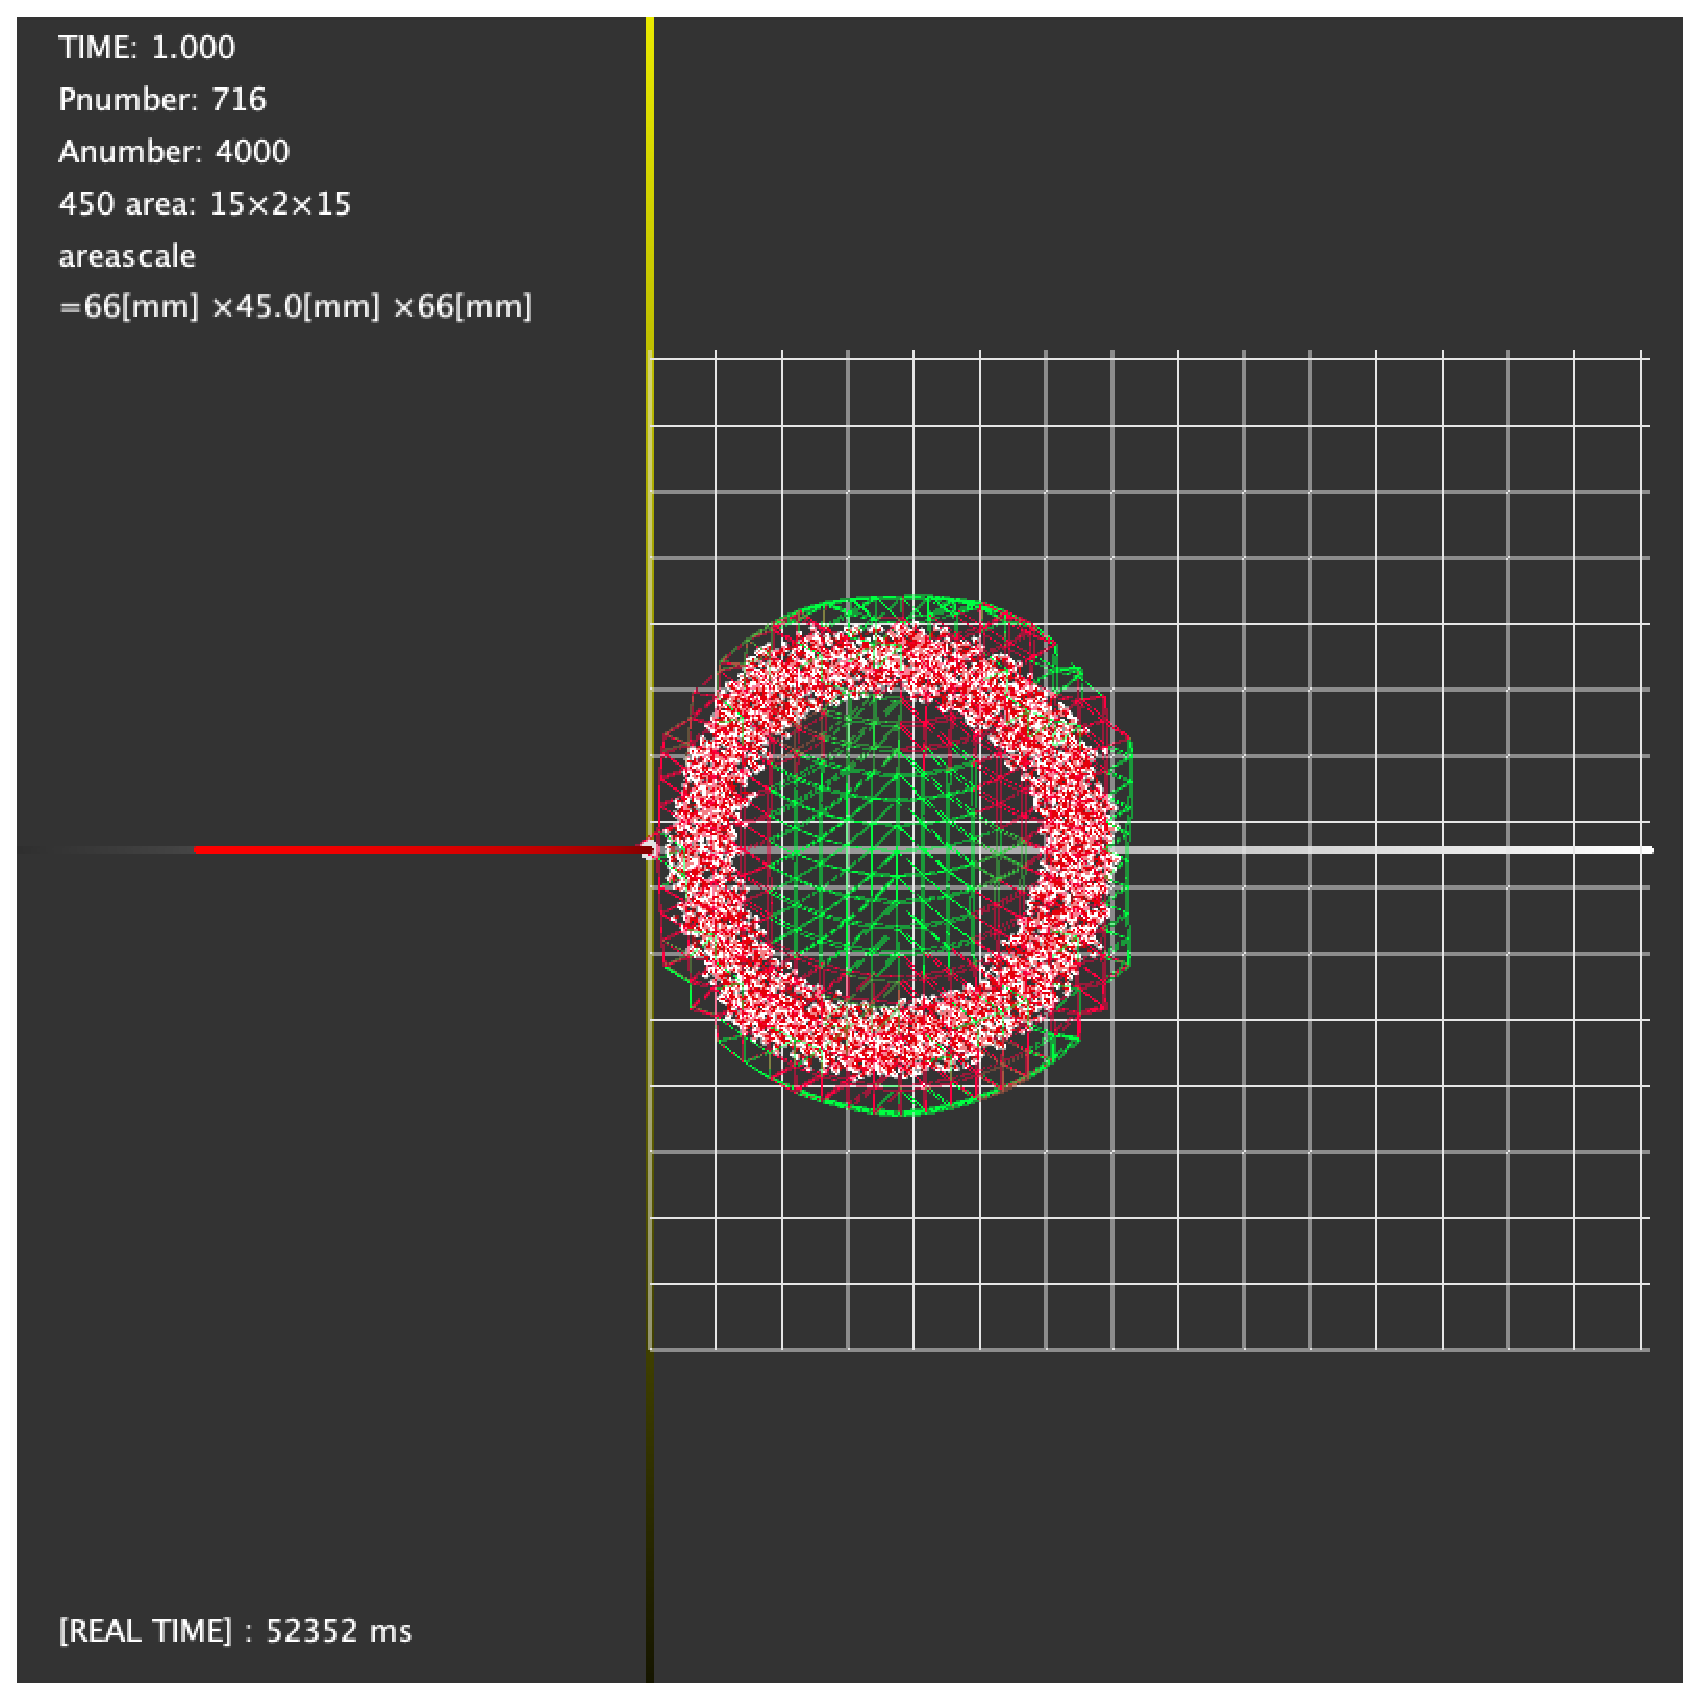
\includegraphics[width=5cm]{top10_ci.eps} 
  \end{tabular}
 }%
 \subfloat[]{%
  \begin{tabular}{c}
   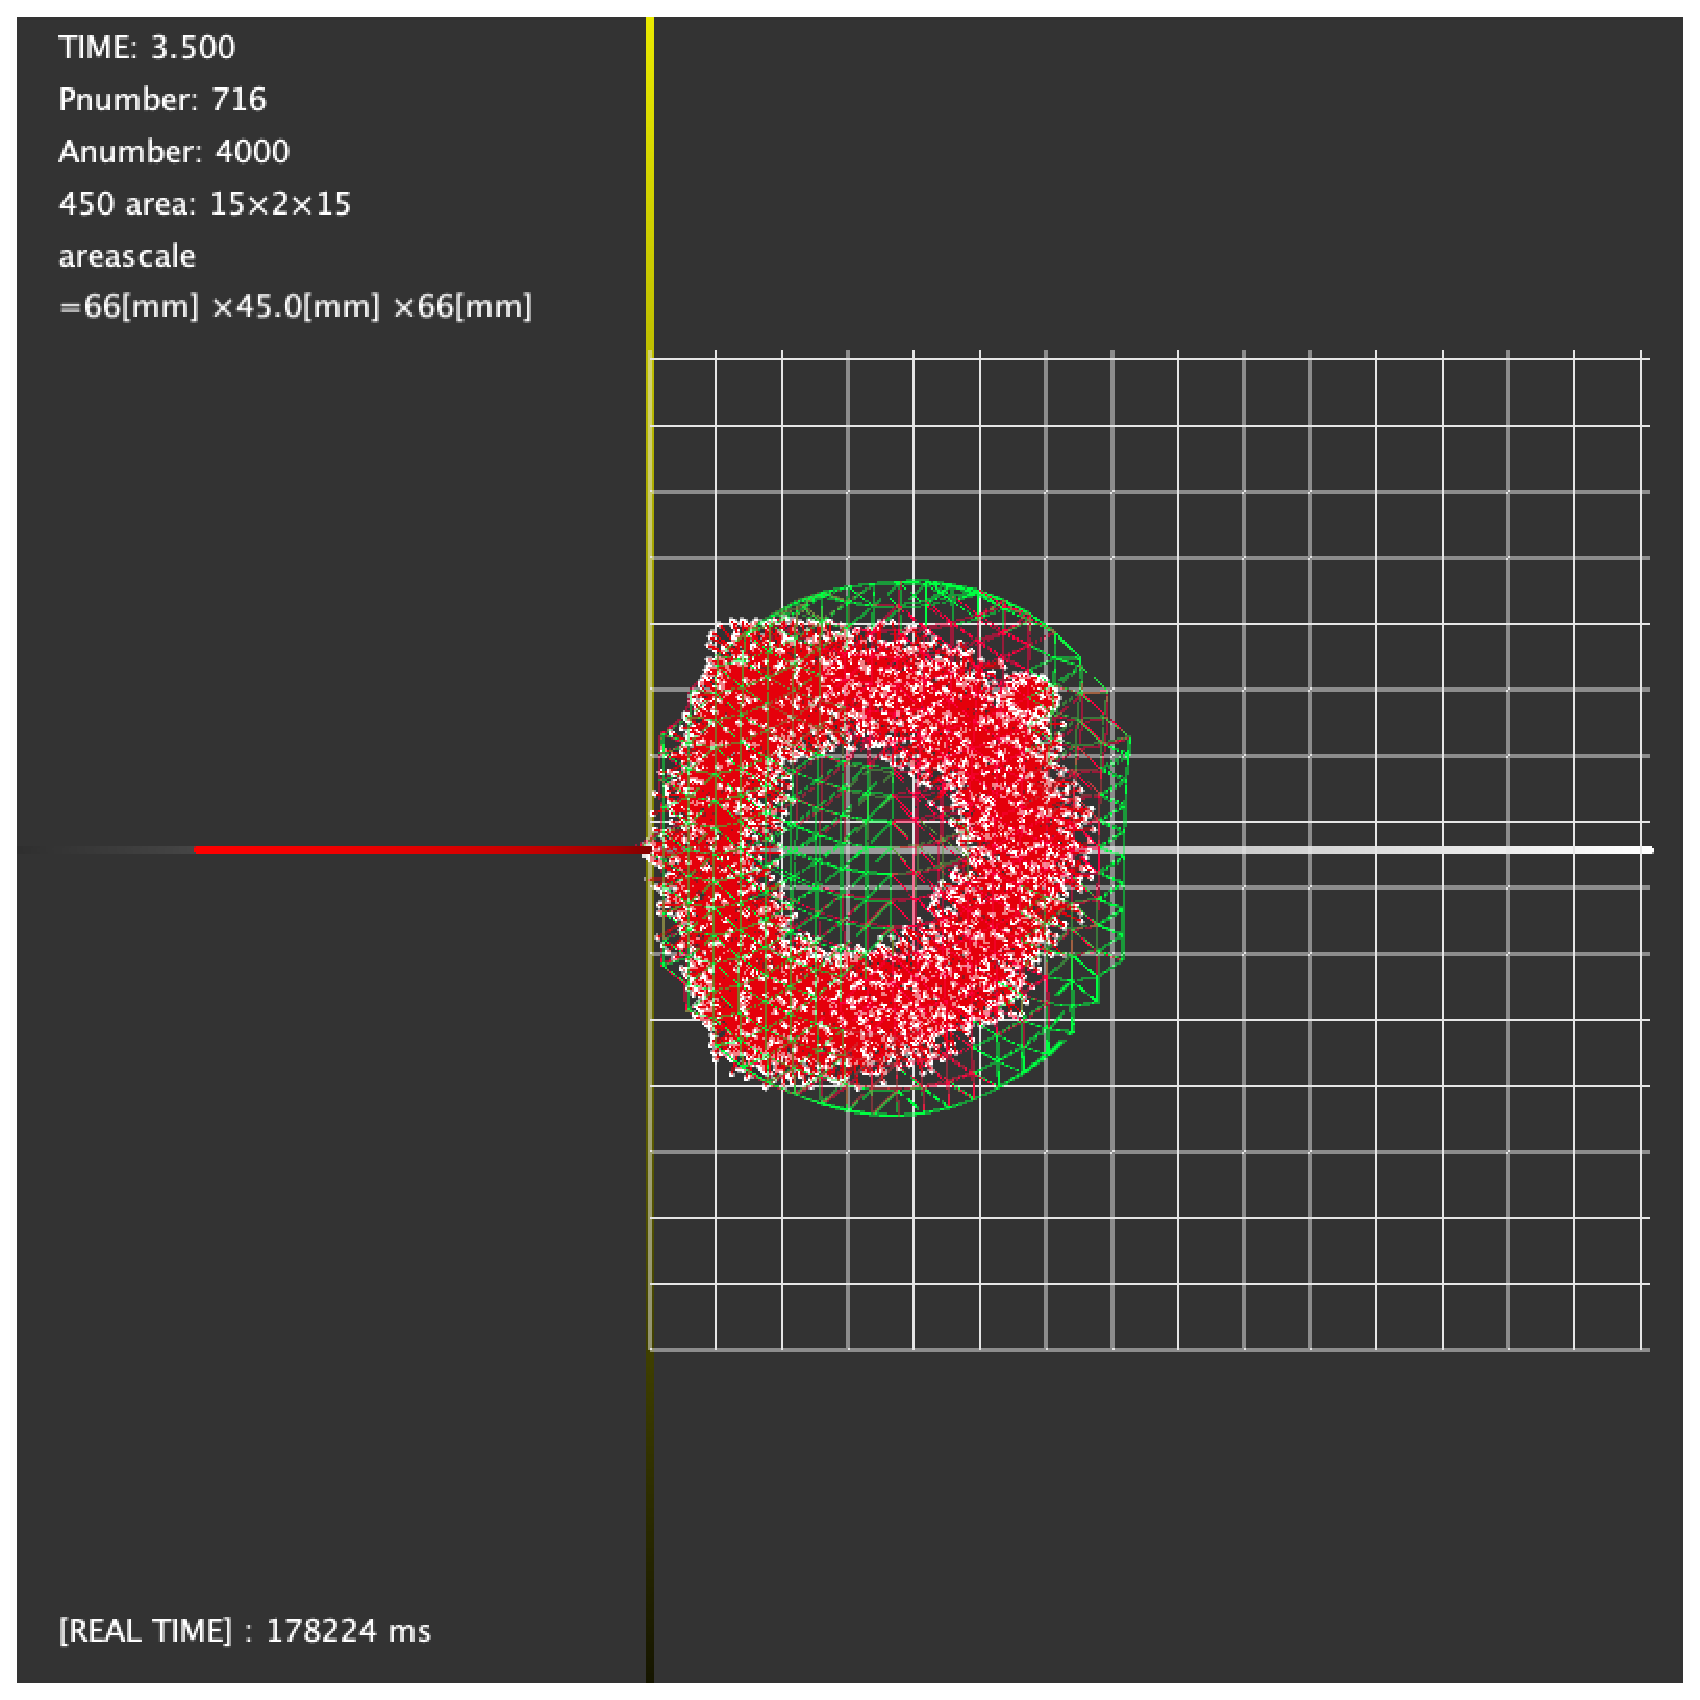
\includegraphics[width=5cm]{top35_ci.eps} 
  \end{tabular}
 }%
 \subfloat[]{%
  \begin{tabular}{c}
   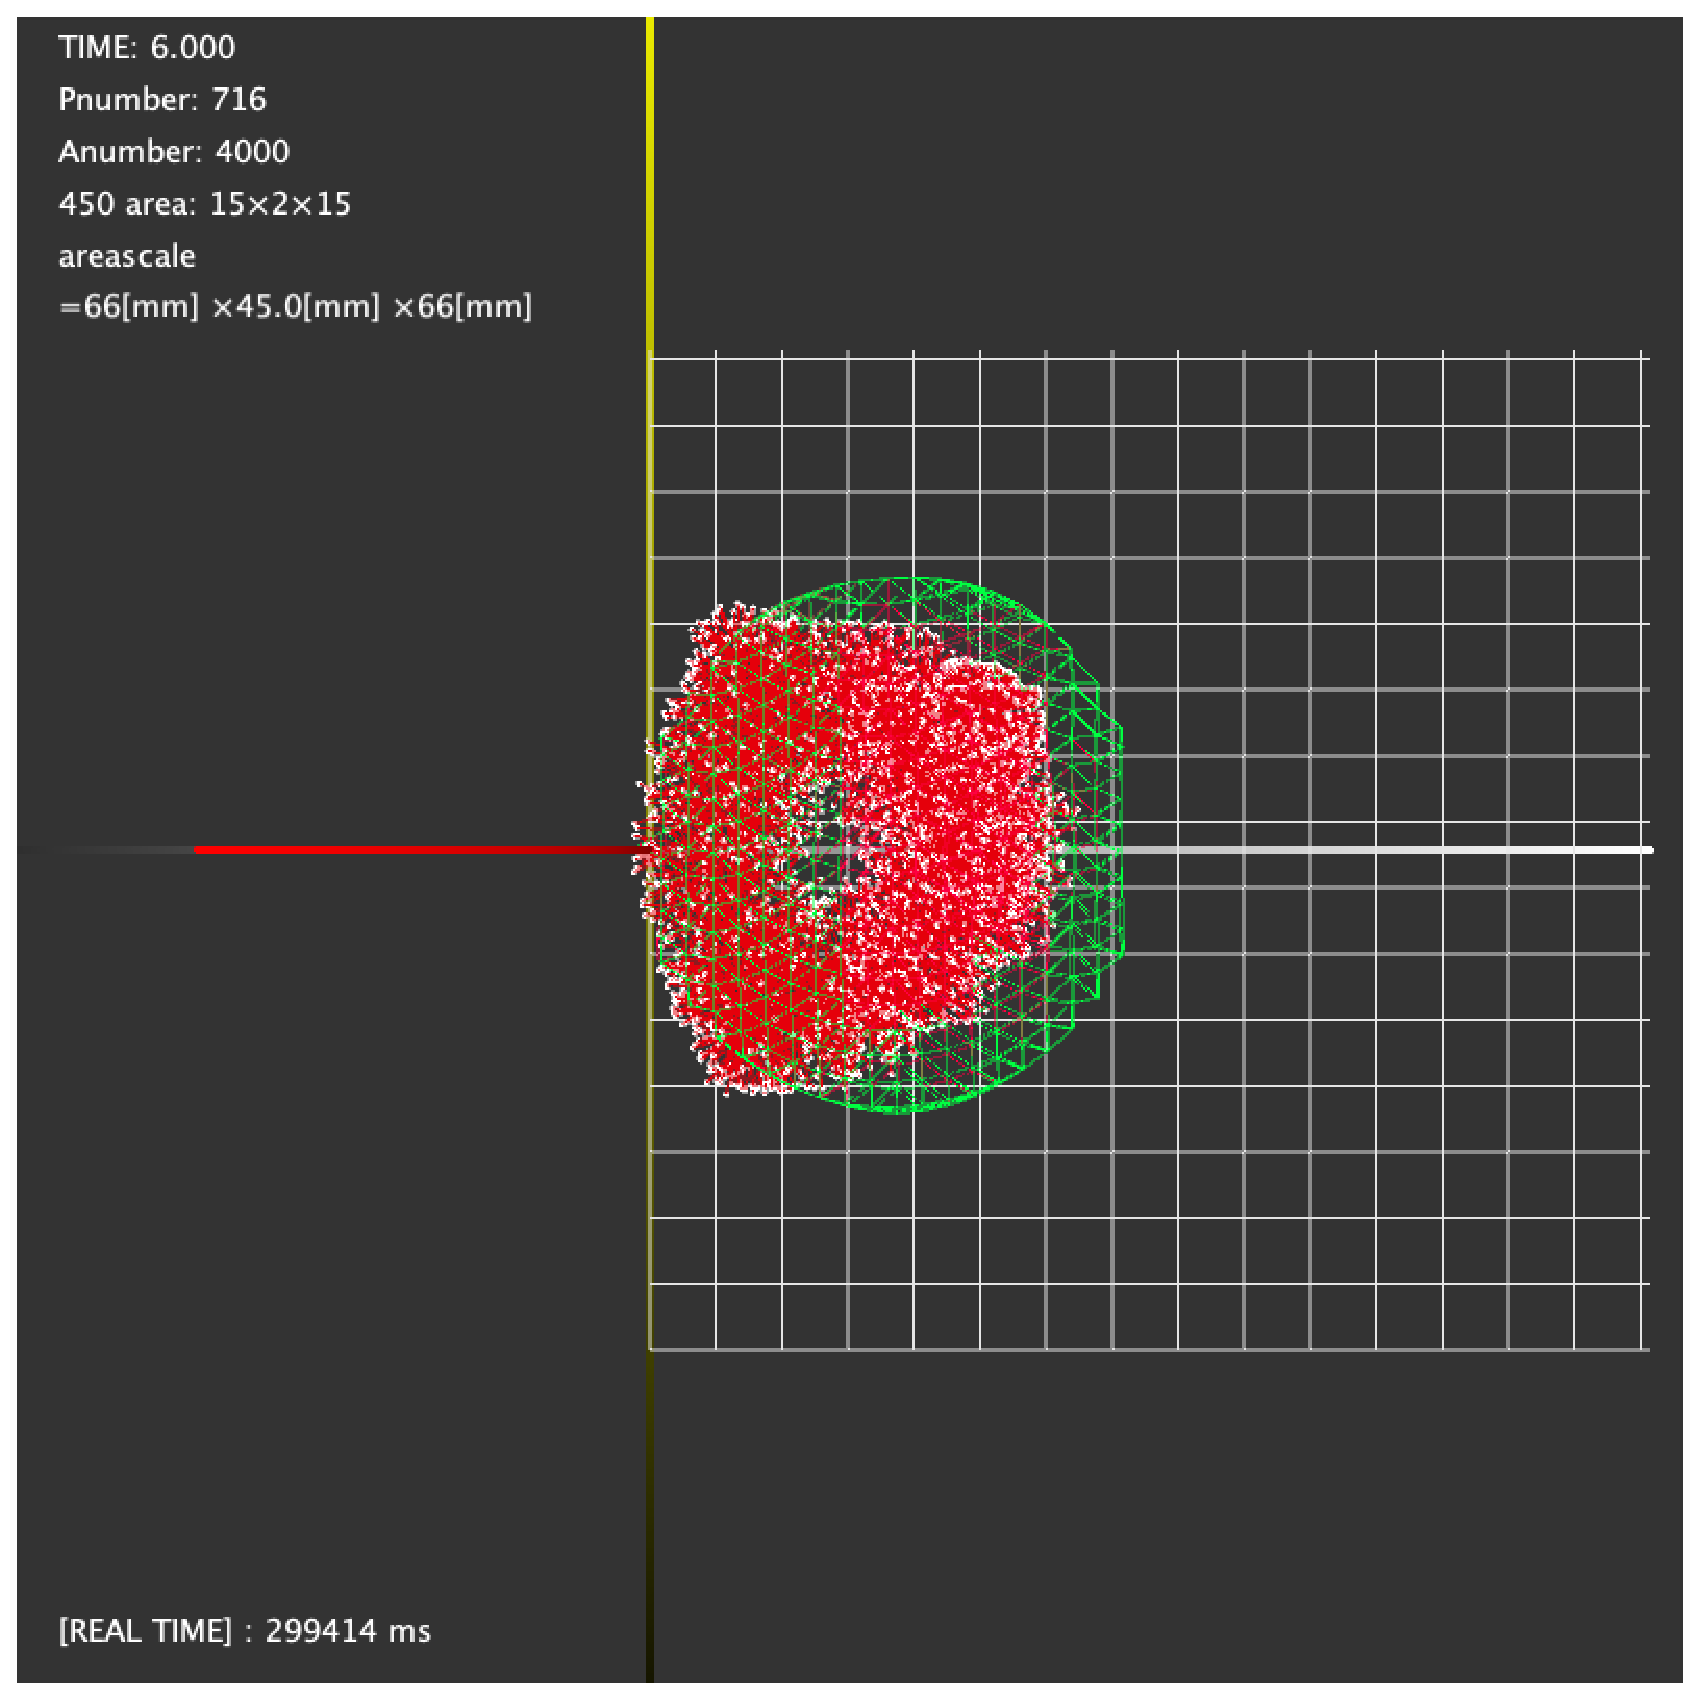
\includegraphics[width=5cm]{top60_ci.eps} 
  \end{tabular}
 }%
 \caption{Simulation results when actin molecules are distributed in a circular region as an initial condition.}
 \label{fig:res4}
\end{figure}


The initial arrangement of actin molecules was half donut-shaped, but simulations were carried out for other shapes (Fig.\ref{fig:res4}). Since it is not a half donut type, since the distribution of the actin molecule is not biased, the direction of cell movement was not determined. Moreover, since the effect of ARF affects actin molecule, the aggregation occurs near SF.

\section{Discussion}
The cell membrane molecule undergoes both the force from the actin molecule and the force of the nearby membrane molecule simultaneously.
Therefore, when the actin molecule is excessively polymerized, the cell membrane can not be flexibly deformed, so it ruptures. 
This result suggests that ARF alleviates the excessive load on the cell membrane by regressing actin molecule.
However, as ARF continually pulls actin molecules, it eventually inhibits the effect on cell membranes.
As can be seen from Fig.\ref{fig:res4}, in the case where ARF exists from a state in which the distribution of actin molecules is unbiased, a half-moon shape is not formed.
The ARF is not constant, and it is presumed that the intensity of influence will change as time passes.
As cell migration progresses SF is gradually formed and ARF is considered to occur.
As can be seen from comparison between Fig.\ref{fig:res0} and Fig.\ref{fig:res2}, actin molecules aggregate in a half-moon shape when ARF occurs from SF.
SF is an actomyosin bundle formed by depolymerized actin molecule accumulating in the posterior part and combining with myosin molecule.
As SF does not exist in the initial state, it is presumed that ARF probably also does not exist at the initial stage of cell migration.

If the actin molecule is located far away from the SF, there may be a mechanism that weakens or inhibit ARF.
This is because if the strength of ARF is constant, the influence of AP does not pass well to the cell membrane.

\chapter{Conclusion}
\section{Conclusion}
Actin molecules played an important role in migrating cells. The actin molecule is attracted in the direction opposite to the polymerization direction by ARF caused by SF while pushing the cell membrane while approaching the cell membrane while repeating polymerization and depolymerization. AP and ARF are intracellular mechanisms acting in opposite directions, respectively. However, if either mechanism is lacking, a half-moon shaped form is not formed. Cell migration is a complicated combination of these two elements.

ARF changes the direction of polymerization when drawing actin molecules towards SF.
It is presumed that the form formed differs depending on how much the angle changes at this time.
It was suggested that the effect of aligning the orientation of the AP to the direction of the ARF is important for the formation of the half-moon shape and that the contraction effect of the actin molecule prevents excessive expansion of the cell membrane.

In this study, it is assumed that both ends of SF are pulling actin molecules, but it is considered that the form formed is different under other conditions.
Therefore, the form formed when precondition is combined with AP condition and ARF condition is half moon shape.

\section{Future Works}
In cell membrane molecular simulation, we could not cope with the movement of actin molecule well. Even if the actin molecule polymerized at the front pushes the cell membrane, the displacement of the membrane molecule is slow to propagate to the back.
\chapter*{Acknowledgements}
I would like to thank Prof. Nishii whose enormous support and insightful comments were invaluable during the course of my study. I also owe a very important debt to Prof. Urakami, Prof. Iwadate and the members of the laboratory whose comments made an enormous contribution to my work. 

\addcontentsline{toc}{chapter}{Acknowledgements}
\bibliography{bibtexfile.bib}
\bibliographystyle{junsrt}

\addcontentsline{toc}{chapter}{\bibname}
\end{document}
